% Options for packages loaded elsewhere
\PassOptionsToPackage{unicode}{hyperref}
\PassOptionsToPackage{hyphens}{url}
%
\documentclass[
  ignorenonframetext,
  serif,
  professionalfont,
  usenames,
  dvipsnames,
  aspectratio = 169]{beamer}
\usepackage{pgfpages}
\setbeamertemplate{caption}[numbered]
\setbeamertemplate{caption label separator}{: }
\setbeamercolor{caption name}{fg=normal text.fg}
\beamertemplatenavigationsymbolsempty
% Prevent slide breaks in the middle of a paragraph
\widowpenalties 1 10000
\raggedbottom
\setbeamertemplate{part page}{
  \centering
  \begin{beamercolorbox}[sep=16pt,center]{part title}
    \usebeamerfont{part title}\insertpart\par
  \end{beamercolorbox}
}
\setbeamertemplate{section page}{
  \centering
  \begin{beamercolorbox}[sep=12pt,center]{part title}
    \usebeamerfont{section title}\insertsection\par
  \end{beamercolorbox}
}
\setbeamertemplate{subsection page}{
  \centering
  \begin{beamercolorbox}[sep=8pt,center]{part title}
    \usebeamerfont{subsection title}\insertsubsection\par
  \end{beamercolorbox}
}
\AtBeginPart{
  \frame{\partpage}
}
\AtBeginSection{
  \ifbibliography
  \else
    \frame{\sectionpage}
  \fi
}
\AtBeginSubsection{
  \frame{\subsectionpage}
}
\usepackage{amsmath,amssymb}
\usepackage{lmodern}
\usepackage{iftex}
\ifPDFTeX
  \usepackage[T1]{fontenc}
  \usepackage[utf8]{inputenc}
  \usepackage{textcomp} % provide euro and other symbols
\else % if luatex or xetex
  \usepackage{unicode-math}
  \defaultfontfeatures{Scale=MatchLowercase}
  \defaultfontfeatures[\rmfamily]{Ligatures=TeX,Scale=1}
\fi
% Use upquote if available, for straight quotes in verbatim environments
\IfFileExists{upquote.sty}{\usepackage{upquote}}{}
\IfFileExists{microtype.sty}{% use microtype if available
  \usepackage[]{microtype}
  \UseMicrotypeSet[protrusion]{basicmath} % disable protrusion for tt fonts
}{}
\makeatletter
\@ifundefined{KOMAClassName}{% if non-KOMA class
  \IfFileExists{parskip.sty}{%
    \usepackage{parskip}
  }{% else
    \setlength{\parindent}{0pt}
    \setlength{\parskip}{6pt plus 2pt minus 1pt}}
}{% if KOMA class
  \KOMAoptions{parskip=half}}
\makeatother
\usepackage{xcolor}
\newif\ifbibliography
\usepackage{longtable,booktabs,array}
\usepackage{calc} % for calculating minipage widths
\usepackage{caption}
% Make caption package work with longtable
\makeatletter
\def\fnum@table{\tablename~\thetable}
\makeatother
\usepackage{graphicx}
\makeatletter
\def\maxwidth{\ifdim\Gin@nat@width>\linewidth\linewidth\else\Gin@nat@width\fi}
\def\maxheight{\ifdim\Gin@nat@height>\textheight\textheight\else\Gin@nat@height\fi}
\makeatother
% Scale images if necessary, so that they will not overflow the page
% margins by default, and it is still possible to overwrite the defaults
% using explicit options in \includegraphics[width, height, ...]{}
\setkeys{Gin}{width=\maxwidth,height=\maxheight,keepaspectratio}
% Set default figure placement to htbp
\makeatletter
\def\fps@figure{htbp}
\makeatother
\setlength{\emergencystretch}{3em} % prevent overfull lines
\providecommand{\tightlist}{%
  \setlength{\itemsep}{0pt}\setlength{\parskip}{0pt}}
\setcounter{secnumdepth}{-\maxdimen} % remove section numbering
% Definição do esquema de cores:
% 1. UFPR - Azul com cinza.
% 2. DEST - Roxo com cinza.
% 3. LEG - Laranjado com cinza.
\def\mycolorscheme{1}

% Caminho para a imagem de fundo com aspecto 16x9.
% \def\pathtobg{config/ufpr-fachada-baixo-1.jpg}
% \def\pathtobg{config/ufpr-fundo.jpg}
% \def\pathtobg{config/ufpr-fundo.jpg}
\def\pathtobg{./config/ufpr-fundo-16x9.jpg}

% \providecommand{\tightlist}{%
%   \setlength{\itemsep}{0pt}\setlength{\parskip}{0pt}}
% ATTENTION: Redefine o comando acima que é definido pelo template.
% \renewcommand{\tightlist}{}
\renewcommand{\tightlist}{%
  \setlength{\itemsep}{0\baselineskip}
  \setlength{\parskip}{0.25\baselineskip}
}

% Logo na capa.
\titlegraphic{
  %\vspace{-1em}
  %\includegraphics[height=1.2cm]{config/dest-texto-2.png}\hspace{1em}
  %\includegraphics[height=1.8cm]{config/dsbd-logo-2x2.png}\hspace{1em}
  
\includegraphics[height=1.8cm]{config/ufpr-transparent-600px.png}
}
%-----------------------------------------------------------------------

% Palladio.
% \usepackage[sc]{mathpazo}
% \linespread{1.05}         % Palladio needs more leading (space between lines)
% \usepackage[T1]{fontenc}

% Kurier.
% \usepackage[light, condensed, math]{kurier}
% \usepackage[T1]{fontenc}

% Iwona.
% \usepackage[math, light, condensed]{iwona}

% \usepackage{cmbright}
% \usepackage[charter]{mathdesign}
% \usepackage{palatino}

% Roboto (with Iwona for maths).
% \usepackage[math]{iwona}
% \usepackage[sfdefault, light, condensed]{roboto}

% Source Sans Pro (with Iwona for maths).
% \usepackage[math]{iwona}
% \usepackage[default, light]{sourcesanspro}

% Lato (with Iwona for maths).
% \usepackage[math]{iwona}
% \usepackage[default]{lato}

% Fira Sans (with Iwona for maths).
\usepackage[math, light]{iwona}
\usepackage[sfdefault,light]{FiraSans} %% option 'sfdefault' activates Fira Sans as the default text font
\usepackage[T1]{fontenc}
\renewcommand*\oldstylenums[1]{{\firaoldstyle #1}}

% Font for code. ----------------------------
% \usepackage[scaled=.75]{beramono}
\usepackage{inconsolata}

% ATTENTION: needs complile with xelatex: `$ xelatex file.tex`
% \usepackage{fontspec}
% \setmonofont{M+ 1m}
% \setmonofont{M+ 1mn}
% \setmonofont{M+ 2m}

%-----------------------------------------------------------------------

% \usepackage{lmodern}
\usepackage{amssymb, amsmath}
\usepackage[makeroom]{cancel}
% \usepackage{ifxetex, ifluatex}
\usepackage{fixltx2e} % provides \textsubscript
\usepackage[utf8]{inputenc}
\usepackage[shorthands=off,main=brazil]{babel}
\usepackage{graphicx}
\usepackage{xcolor}
\usepackage{setspace}
\usepackage{comment}
\usepackage{icomma}

%-----------------------------------------------------------------------
% Algumas configurações.

\setlength{\parindent}{0pt}
\setlength{\parskip}{6pt plus 2pt minus 1pt}
\setlength{\emergencystretch}{3em}  % prevent overfull lines
% \providecommand{\tightlist}{%
%   \setlength{\itemsep}{0pt}\setlength{\parskip}{0pt}}
\setcounter{secnumdepth}{0}

% Espaço vertical para o ambiente `quote`.
\let\oldquote\quote
\let\oldendquote\endquote
\renewenvironment{quote}{%
  \vspace{1em}\oldquote}{%
  \oldendquote\vspace{1em}}

%-----------------------------------------------------------------------
% Espaçamento entre items para itemize, enumerate e description.

% % itemize.
% \let\itemopen\itemize
% \let\itemclose\enditemize
% \renewenvironment{itemize}{%
%   \itemopen\addtolength{\itemsep}{0.25\baselineskip}}{\itemclose}
%
% % enumerate.
% \let\enumopen\enumerate
% \let\enumclose\endenumerate
% \renewenvironment{enumerate}{%
%   \enumopen\addtolength{\itemsep}{0.25\baselineskip}}{\enumclose}
%
% % description.
% \let\descopen\description
% \let\descclose\enddescription
% \renewenvironment{description}{%
%   \descopen\addtolength{\itemsep}{0.25\baselineskip}}{\descclose}

%-----------------------------------------------------------------------

% \usepackage[hang]{caption}
\usepackage{caption}
\captionsetup{font=footnotesize,
  labelfont={color=mycolor1, footnotesize},
  labelsep=period}

% \providecommand{\tightlist}{%
%   \setlength{\itemsep}{0pt}\setlength{\parskip}{0pt}}

%-----------------------------------------------------------------------

\usepackage{tikz}

% \def\pathtobg{/home/walmes/Projects/templates/COMMON/ufpr-fundo.jpg}
% \def\pathtobg{/home/walmes/Projects/templates/COMMON/ufpr-fundo-16x9.jpg}
% \def\pathtobg{/home/walmes/Projects/templates/COMMON/ufpr-fachada-dir-1.jpg}
% \def\pathtobg{/home/walmes/Projects/templates/COMMON/ufpr-fachada-esq-1.jpg}
% \def\pathtobg{/home/walmes/Projects/templates/COMMON/ufpr-perto-1.jpg}
% \def\pathtobg{/home/walmes/Projects/templates/COMMON/ufpr-fachada-baixo-1.jpg}

\ifx\pathtobg\undefined
\else
  \usebackgroundtemplate{
    \tikz[overlay, remember picture]
    \node[% opacity=0.3,
          at=(current page.south east),
          anchor=south east,
          inner sep=0pt] {
            \includegraphics[height=\paperheight, width=\paperwidth]{\pathtobg}};
  }
\fi

%-----------------------------------------------------------------------
% Definições de esquema de cores.

\ifx\mycolorscheme\undefined
  % UFPR.
  % http://www.color-hex.com/color-palette/2018
  \definecolor{mycolor1}{HTML}{015c93} % Título.
  \definecolor{mycolor2}{HTML}{363435} % Texto.
  \definecolor{mycolor3}{HTML}{015c93} % Estrutura.
  \definecolor{mycolor4}{HTML}{015c93} % Links.
  \definecolor{mycolor5}{HTML}{CECAC5} % Preenchimentos.
\else
  \if\mycolorscheme1
    % UFPR.
    \definecolor{mycolor1}{HTML}{015c93} % Título.
    \definecolor{mycolor2}{HTML}{363435} % Texto.
    \definecolor{mycolor3}{HTML}{015c93} % Estrutura.
    \definecolor{mycolor4}{HTML}{015c93} % Links.
    \definecolor{mycolor5}{HTML}{CECAC5} % Preenchimentos.
  \fi
  \if\mycolorscheme2
    % DEST.
    \definecolor{mycolor1}{HTML}{2a0e72} % Título.
    \definecolor{mycolor2}{HTML}{202E35} % Texto.
    \definecolor{mycolor3}{HTML}{2a0e72} % Estrutura.
    % \definecolor{mycolor3}{HTML}{8072a3} % Estrutura.
    \definecolor{mycolor4}{HTML}{2a0e72} % Links.
    % \definecolor{mycolor4}{HTML}{bfb9d1} % Links.
    % \definecolor{mycolor5}{HTML}{AEA79F} % Preenchimentos.
    \definecolor{mycolor5}{HTML}{CECAC5} % Preenchimentos.
  \fi
  \if\mycolorscheme3
    % LEG.
    \definecolor{mycolor2}{HTML}{363435} % Texto.
    % \definecolor{mycolor1}{HTML}{ff8000} % Título.
    % \definecolor{mycolor3}{HTML}{ff8000} % Estrutura.
    % \definecolor{mycolor4}{HTML}{ff8000} % Links.
    % \definecolor{mycolor1}{HTML}{E57300} % Título.
    % \definecolor{mycolor3}{HTML}{E57300} % Estrutura.
    % \definecolor{mycolor4}{HTML}{E57300} % Links.
    \definecolor{mycolor1}{HTML}{F67014} % Título.
    \definecolor{mycolor3}{HTML}{F67014} % Estrutura.
    \definecolor{mycolor4}{HTML}{F67014} % Links.
    % \definecolor{mycolor1}{HTML}{FE5C23} % Título.
    % \definecolor{mycolor3}{HTML}{FE5C23} % Estrutura.
    % \definecolor{mycolor4}{HTML}{FE5C23} % Links.
    \definecolor{mycolor5}{HTML}{222222} % Preenchimentos.
    \definecolor{mycolor5}{HTML}{383838} % Preenchimentos.
  \fi
\fi

\hypersetup{
  colorlinks=true,
  linkcolor=mycolor4,
  urlcolor=mycolor1,
  citecolor=mycolor1
}

%-----------------------------------------------------------------------
% ATTENTION: http://www.cpt.univ-mrs.fr/~masson/latex/Beamer-appearance-cheat-sheet.pdf

\usetheme{Boadilla}
\usecolortheme{default}

% \setbeamersize{text margin left=7mm, text margin right=7mm}
% \setbeamertemplate{frametitle}[default][left, leftskip=3mm]
% \addtobeamertemplate{frametitle}{\vspace{0.5em}}{}

\setbeamertemplate{caption}[numbered]
\setbeamertemplate{section in toc}[sections numbered]
\setbeamertemplate{subsection in toc}[subsections numbered]
\setbeamertemplate{sections/subsections in toc}[ball]{}
\setbeamertemplate{sections in toc}[ball]
\setbeamercolor{section number projected}{bg=mycolor1, fg=white}
\setbeamertemplate{blocks}[rounded]
\setbeamertemplate{navigation symbols}{}
\setbeamertemplate{frametitle continuation}{\gdef\beamer@frametitle{}}
% \setbeamertemplate{frametitle}[default][center]
% \setbeamertemplate{footline}[frame number]

\setbeamertemplate{enumerate items}[default]
\setbeamertemplate{itemize items}{\scriptsize\raise1.25pt\hbox{\donotcoloroutermaths$\blacktriangleright$}}

% Blocos.
% \addtobeamertemplate{block begin}{\vskip -\bigskipamount}{}
% \addtobeamertemplate{block end}{}{\vskip -\bigskipamount}
\addtobeamertemplate{block begin}{\vspace{0.5em}}{}
\addtobeamertemplate{block end}{}{\vspace{0.5em}}


% Rodapé.
\setbeamercolor{title in head/foot}{parent=subsection in head/foot}
\setbeamercolor{author in head/foot}{bg=mycolor4, fg=white}
\setbeamercolor{date in head/foot}{parent=subsection in head/foot, fg=mycolor3}

% Cabeçalho.
\setbeamercolor{section in head/foot}{bg=mycolor2, fg=mycolor4}
\setbeamercolor{subsection in head/foot}{bg=mycolor2, fg=white}

\setbeamercolor{title}{fg=mycolor1}       % Título dos slides.
\setbeamercolor{titlelike}{fg=title}
\setbeamercolor{subtitle}{fg=mycolor2}    % Subtítulo.
\setbeamercolor{institute in head/foot}{parent=palette primary} % Instituição.
\setbeamercolor{frametitle}{fg=mycolor1}  % De quadro.
\setbeamercolor{structure}{fg=mycolor3}   % Listas e rodapé.
\setbeamercolor{item projected}{bg=mycolor2}
\setbeamercolor{block title}{bg=mycolor5, fg=mycolor2}
\setbeamercolor{normal text}{fg=mycolor2} % Texto.
\setbeamercolor{caption name}{fg=normal text.fg}
% \setbeamercolor{footlinecolor}{fg=mycolor2, bg=mycolor5}
% \setbeamercolor{section in head/foot}{fg=mycolor2, bg=mycolor5}
\setbeamercolor{author in head/foot}{fg=white, bg=mycolor1}
\setbeamercolor{section in foot}{fg=mycolor4, bg=mycolor5}
\setbeamercolor{date in foot}{fg=mycolor4, bg=mycolor5}
\setbeamercolor{block title}{fg=white, bg=mycolor1}
\setbeamercolor{block body}{fg=black, bg=white!80!gray}
\setbeamercolor{block body}{fg=black, bg=white!80!gray}

% To remove empty brackets of \institution.
\makeatletter
\setbeamertemplate{footline}{
  \leavevmode%
  \hbox{%
    \begin{beamercolorbox}[
      wd=0.3\paperwidth, ht=2.25ex, dp=1ex, right]{author in head/foot}%
      \usebeamerfont{author in head/foot}\insertshortauthor{}\hspace*{1ex}
    \end{beamercolorbox}%
    \begin{beamercolorbox}[
      wd=0.6\paperwidth, ht=2.25ex, dp=1ex, left]{section in foot}%
      \usebeamerfont{title in head/foot}\hspace*{1ex}\insertshorttitle{}
      % \usebeamerfont{title in head/foot}\hspace*{1ex}\insertframetitle{}
    \end{beamercolorbox}%
    \begin{beamercolorbox}[
      wd=0.1\paperwidth, ht=2.25ex, dp=1ex, right]{date in foot}%
      \insertframenumber{}\hspace*{2ex}
    \end{beamercolorbox}
  }%
  \vskip0pt%
}
\makeatother

%-----------------------------------------------------------------------

% \usepackage{hyphenat}
\usepackage{changepage}

% Slide para o título das seções.
\AtBeginSection[]{
  \begin{frame}
    % \vfill
    \vspace{4cm}
    % \centering
    % \begin{beamercolorbox}[sep = 8pt, center, shadow = true, rounded = true]{title}
    \begin{beamercolorbox}{title}
      \begin{columns}
        \column{0.7\linewidth}
        {\LARGE\textbf \insertsectionhead}
      \end{columns}
    \end{beamercolorbox}
    \vfill
  \end{frame}
}

%-----------------------------------------------------------------------
%---- preamble-chunk.tex -----------------------------------------------

% Knitr.

% ATTENTION: this needs `\usepackage{xcolor}'.
\definecolor{color_line}{HTML}{333333}
\definecolor{color_back}{HTML}{DDDDDD}
% \definecolor{color_back}{HTML}{FF0000}

% ATTENTION: usa o fancyvrb.
% https://ctan.math.illinois.edu/macros/latex/contrib/fancyvrb/doc/fancyvrb-doc.pdf
% R input.
\usepackage{tcolorbox}
\ifcsmacro{Highlighting}{
  % Statment if it exists. ------------------
  \DefineVerbatimEnvironment{Highlighting}{Verbatim}{
    % frame=lines,     % Linha superior e inferior.
    % framerule=0.5pt, % Espessura da linha.
    framesep=2ex,    % Distância da linha para o texto.
    % rulecolor=\color{color_line},
    % numbers=right,
    fontsize=\footnotesize, % Tamanho da fonte.
    baselinestretch=0.8,    % Espaçamento entre linhas.
    commandchars=\\\{\}}
  % Margens do ambiente `Shaded'.
  % \fvset{listparameters={\setlength{\topsep}{-1em}}}
  % \renewenvironment{Shaded}{\vspace{-1ex}}{\vspace{-2ex}}
  \renewenvironment{Shaded}{
    \vspace{2pt}
    \begin{tcolorbox}[
      boxrule=0pt,      % Espessura do contorno.
      colframe=gray!10, % Cor do contorno.
      colback=gray!10,  % Cor de fundo da caixa.
      arc=1em,          % Raio para contornos arredondados.
      sharp corners,
      boxsep=0.5em,     % Margem interna.
      left=3pt, right=3pt, top=3pt, bottom=3pt, % Margens internas.
      grow to left by=0mm,
      grow to right by=6pt,
      ]
    }{
    \end{tcolorbox}
    \vspace{-3pt}
    }
  }{
  % Statment if it not exists. --------------
}

% R output e todo `verbatim'.
\makeatletter
\def\verbatim@font{\linespread{0.8}\ttfamily\footnotesize}
%\makeatother

% Cor de fundo e margens do `verbatim'.
\let\oldv\verbatim
\let\oldendv\endverbatim

\def\verbatim{%
  \par\setbox0\vbox\bgroup % Abre grupo.
  %\vspace{-5px}            % Reduz margem superior.
  \oldv                    % Chama abertura do verbatim.
}
\def\endverbatim{%
  \oldendv                 % Chama encerramento do verbatim.
  %\vspace{0cm}           % Controla margem inferior.
  \egroup%\fboxsep5px      % Fecha grupo.
  \noindent{{\usebox0}}\par
}

%-----------------------------------------------------------------------
%---- preamble-commands.tex --------------------------------------------

% Para fazer texto em duas colunas.
\newcommand{\mytwocolumns}[4]{
  % #1: Line width fraction for the left column , e.g. 0.5.
  % #2: Line width fraction for the right column.
  % #3: Content for the left column.
  % #4: Content for the right column.
  \begin{columns}[c]
    \begin{column}{#1\linewidth} %----------- left.
      #3
    \end{column} %--------------------------- left.
    \begin{column}{#2\linewidth} %----------- right.
      #4
    \end{column} %--------------------------- right.
  \end{columns}
}

%-----------------------------------------------------------------------
% Para fazer duas colunas no Rmd.

% Center vertical align.
\def\beginAHalfColumn{\begin{minipage}{0.49\textwidth}}%
\def\beginAlmostHalfColumn{\begin{minipage}{0.45\textwidth}}%
\def\beginAQuarterColumn{\begin{minipage}{0.23\textwidth}}%
\def\beginThreeQuartersColumn{\begin{minipage}{0.72\textwidth}}%
\def\beginAThirdColumn{\begin{minipage}{0.31\textwidth}}%
\def\beginTwoThirdsColumn{\begin{minipage}{0.64\textwidth}}%
\def\endColumns{\end{minipage}}%

% Top vertical align.
\def\beginAHalfColumnT{\begin{minipage}[t]{0.49\textwidth}}%
\def\beginAlmostHalfColumnT{\begin{minipage}[t]{0.45\textwidth}}%
\def\beginAQuarterColumnT{\begin{minipage}[t]{0.23\textwidth}}%
\def\beginThreeQuartersColumnT{\begin{minipage}[t]{0.72\textwidth}}%
\def\beginAThirdColumnT{\begin{minipage}[t]{0.31\textwidth}}%
\def\beginTwoThirdsColumnT{\begin{minipage}[t]{0.64\textwidth}}%

%---------------------------------------------------------------------
% Ambientes para frases como e sem imagem.

\newcommand{\myquote}[3]{
  % #1: caminho para a imagem.
  % #2: a frase/quotation.
  % #3: o autor.
  \begin{center}
    \begin{minipage}[c]{0.19\linewidth}
      \begin{center}
        \includegraphics[height=2.5cm]{#1}
      \end{center}
    \end{minipage}
    \begin{minipage}[c]{0.7\linewidth}
      \begin{flushright}
        \textit{#2}
        \vspace{1ex}

        -- #3
      \end{flushright}
    \end{minipage}
  \end{center}
}

\newcommand{\myphrase}[2]{
  % #1: a frase/quotation.
  % #2: o autor.
  \begin{center}
    \begin{minipage}[c]{0.19\linewidth}
    \end{minipage}
    \begin{minipage}[c]{0.7\linewidth}
      \begin{flushright}
        \textit{#1}
        \vspace{1ex}

        -- #2
      \end{flushright}
    \end{minipage}
  \end{center}
}

%-----------------------------------------------------------------------
% Comandos para texto em destaque.

% \newcommand{\hi}[1]{%
%   \textcolor{ubuntu_orange}{#1}\xspace
% }

\usepackage{xspace}

% URLs com letra miuda.
\newcommand{\myurl}[1]{%
  {\tiny \url{#1}}\xspace
}

% Botões.
\newcommand{\btn}[1]{%
  \beamergotobutton{#1}\xspace
}

% Texto grande centralizado.
\newcommand{\centertitle}[1]{%
  \begin{center}
    {\LARGE \bfseries \hi{#1}}
  \end{center}
}

%-----------------------------------------------------------------------
\ifLuaTeX
  \usepackage{selnolig}  % disable illegal ligatures
\fi
\IfFileExists{bookmark.sty}{\usepackage{bookmark}}{\usepackage{hyperref}}
\IfFileExists{xurl.sty}{\usepackage{xurl}}{} % add URL line breaks if available
\urlstyle{same} % disable monospaced font for URLs
\hypersetup{
  pdfauthor={Prof.~Me. Lineu Alberto Cavazani de Freitas},
  hidelinks,
  pdfcreator={LaTeX via pandoc}}

\title{\textbf{Análise exploratória I}}
\subtitle{Motivação e análise descritiva univariada para variáveis
qualitativas e quantitativas.}
\author{Prof.~Me. Lineu Alberto Cavazani de Freitas}
\date{}
\institute{\textbf{CE003 – Estatística II}\\
\strut \\
Departamento de Estatística\\
Laboratório de Estatística e Geoinformação}

\begin{document}
\frame{\titlepage}

\begin{frame}{Análise exploratória}
\protect\hypertarget{anuxe1lise-exploratuxf3ria}{}
\begin{itemize}
\item
  Parte primordial de qualquer análise estatística é chamada
  \textbf{análise descritiva} ou \textbf{exploratória}.
\item
  Consiste basicamente de \textbf{tabelas}, \textbf{resumos numéricos} e
  \textbf{análises gráficas} das variáveis disponíveis em um conjunto de
  dados.
\item
  Trata-se de uma etapa de extrema importância e deve preceder qualquer
  análise mais sofisticada.
\item
  As técnicas de análise exploratória visam \textbf{resumir} e
  \textbf{apresentar} as informações de um conjunto de dados brutos.
\end{itemize}
\end{frame}

\begin{frame}{Análise exploratória}
\protect\hypertarget{anuxe1lise-exploratuxf3ria-1}{}
\beginAHalfColumn

\begin{itemize}
\item
  Tentar compreender um conjunto de dados sem algum método que permita
  resumir as informações é inviável.
\item
  A análise exploratória é a primeira forma de tentarmos enteder o que
  acontece nos nossos dados.
\item
  Uma das tarefas é a etapa de consistência dos dados, isto é, verificar
  se os dados coletados são condizentes com a realidade.
\end{itemize}

\endColumns
\beginAHalfColumn

\begin{figure}

{\centering 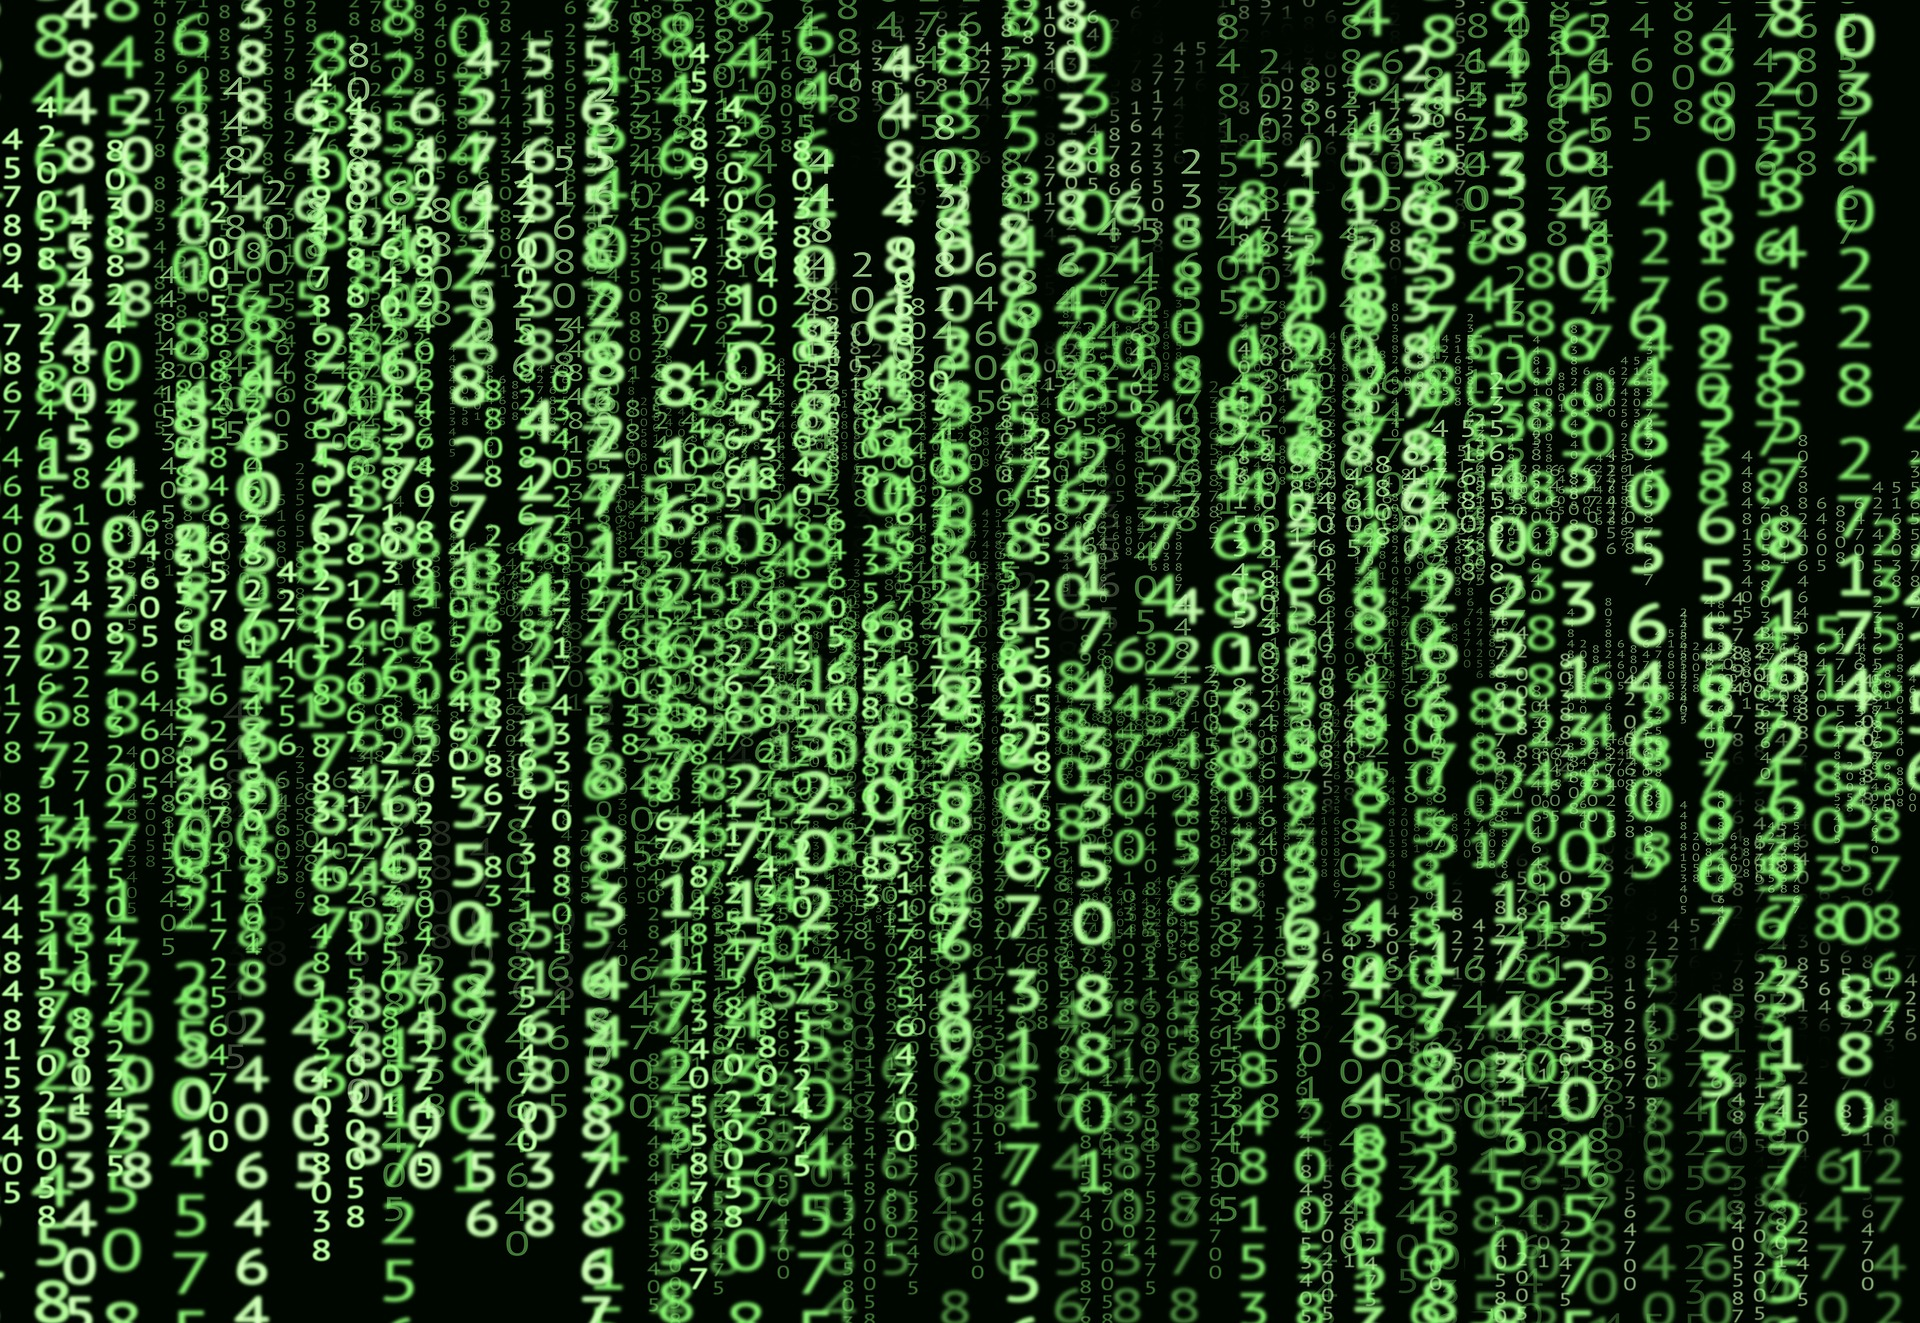
\includegraphics[width=0.9\linewidth]{./img/dados} 

}

\caption{Extraído de \href{https://cdn.pixabay.com/photo/2018/01/26/18/21/matrix-3109378_1280.jpg}{pixabay.com.}}\label{fig:unnamed-chunk-2}
\end{figure}

\endColumns
\end{frame}

\begin{frame}{Análise exploratória}
\protect\hypertarget{anuxe1lise-exploratuxf3ria-2}{}
\beginAHalfColumn

\begin{itemize}
\item
  O conjunto de técnicas aplicáveis está diretamente associado ao
  \textbf{tipo das variáveis de interesse} (quantitativas x
  qualitativas) e suas ramificações.
\item
  Podemos conduzir análises focadas nas variáveis uma a uma
  (\textbf{análises univariadas}).
\item
  Bem como conduzir análises focadas em avaliar a relação entre as
  variáveis (\textbf{análises multivariadas}).
\end{itemize}

\endColumns
\beginAHalfColumn

\begin{figure}

{\centering 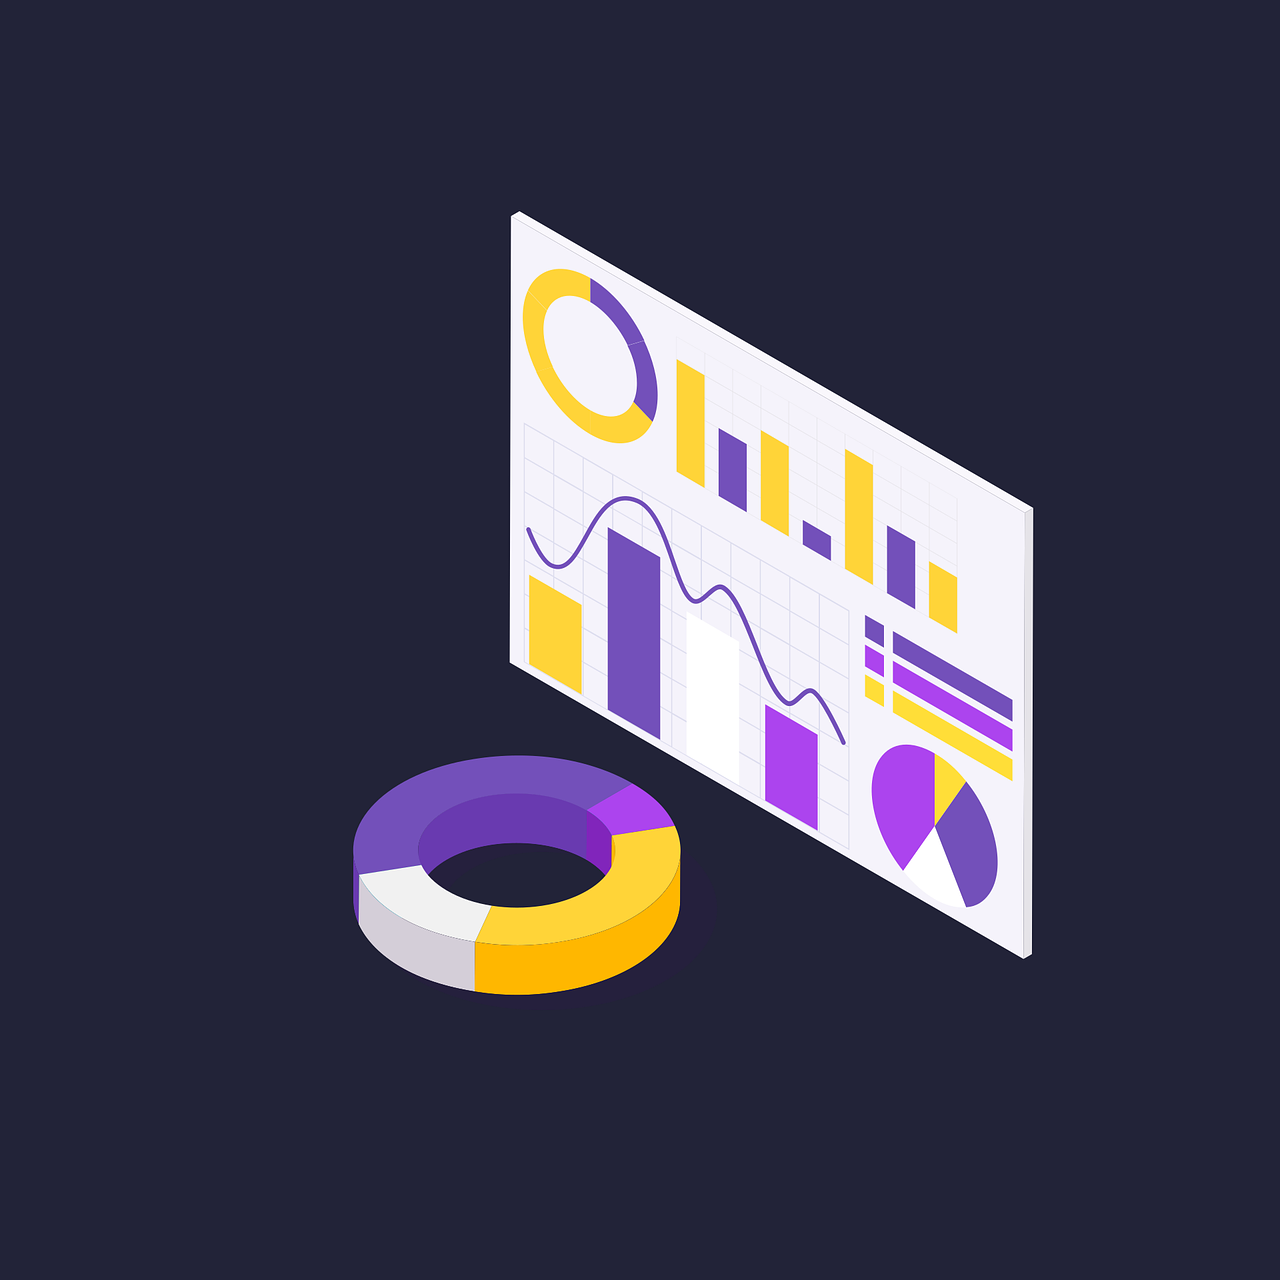
\includegraphics[width=0.8\linewidth]{./img/exploratoria} 

}

\caption{Extraído de \href{https://cdn.pixabay.com/photo/2020/08/03/10/00/graph-5459708_1280.png}{pixabay.com.}}\label{fig:unnamed-chunk-3}
\end{figure}

\endColumns
\end{frame}

\begin{frame}{Análise exploratória}
\protect\hypertarget{anuxe1lise-exploratuxf3ria-3}{}
Podemos fazer uso diversas técnicas, tais como

\beginAHalfColumn

\begin{itemize}
\item
  Tabelas de frequência absolutas.
\item
  Tabelas de frequência relativas.
\item
  Tabelas de frequência acumuladas.
\item
  Tabelas para múltiplas variáveis.
\item
  Gráficos (para análise uni e multivariada).
\end{itemize}

\endColumns
\beginAHalfColumn

\begin{itemize}
\tightlist
\item
  Medidas de posição central.
\item
  Medidas de posição relativa.
\item
  Medidas de forma.
\item
  Medidas de dispersão.
\item
  Medidas de associação.
\end{itemize}

\endColumns
\end{frame}

\hypertarget{anuxe1lise-descritiva-univariada-para-variuxe1veis-qualitativas}{%
\section{Análise descritiva univariada para variáveis
qualitativas}\label{anuxe1lise-descritiva-univariada-para-variuxe1veis-qualitativas}}

\begin{frame}{Análise descritiva univariada para variáveis qualitativas}
\protect\hypertarget{anuxe1lise-descritiva-univariada-para-variuxe1veis-qualitativas-1}{}
\begin{itemize}
\item
  Uma variável qualitativa representa um atributo que pode ser expresso
  por meio de \textbf{rótulos} ou \textbf{categorias}.
\item
  Podem ser classificadas em \textbf{nominais} (sem ordenação natural
  entre os níveis) ou \textbf{ordinais} (com ordenação natural entre os
  níveis).
\item
  As categorias também são chamadas de \textbf{classes} ou
  \textbf{níveis}.
\item
  Na análise descritiva de uma variável qualitativa estamos interessados
  em avaliar as \textbf{frequências} das classes.
\end{itemize}
\end{frame}

\begin{frame}{Tipos de frequência}
\protect\hypertarget{tipos-de-frequuxeancia}{}
\begin{itemize}
\item
  \textbf{Frequência absoluta} (\(f_a\)): número de observações no
  conjunto de dados que pertence a uma determinada classe.
\item
  \textbf{Frequência relativa} (\(f_r\)): frequência de classe dividida
  pelo número total de observações no conjunto de dados.

  \begin{itemize}
  \tightlist
  \item
    Pode ser apresentada em forma de percentual, quando multiplicada por
    100.
  \end{itemize}
\item
  \textbf{Frequência acumulada} (\(F_a\) ou \(F_r\)): frequência
  absoluta ou relativa acumulada conforme disposição das classes.

  \begin{itemize}
  \tightlist
  \item
    Não faz muito sentido para variáveis qualitativas nominais.
  \end{itemize}
\end{itemize}
\end{frame}

\begin{frame}{Tipos de frequência}
\protect\hypertarget{tipos-de-frequuxeancia-1}{}
\textbf{Exemplos}

\beginAHalfColumn

\begin{itemize}
\tightlist
\item
  Frequência absoluta e relativa dos alunos por gênero.

  \begin{itemize}
  \item
    XX do sexo masculino.
  \item
    XX do sexo feminino.
  \item
    \(XX/n = 0,XX\) do sexo masculino (\(XX\%\)).
  \item
    \(XX/n = 0,XX\) do sexo feminino (\(XX\%\)).
  \end{itemize}
\end{itemize}

\endColumns
\beginAHalfColumn

\begin{figure}

{\centering 
\includegraphics[width=0.8\linewidth]{./img/generos2} 

}

\caption{Extraído de \href{https://cdn.pixabay.com/photo/2014/04/03/11/52/gender-312411_1280.png}{pixabay.com.}}\label{fig:unnamed-chunk-4}
\end{figure}

\endColumns
\end{frame}

\begin{frame}{Tabelas de frequência para uma variável qualitativa}
\protect\hypertarget{tabelas-de-frequuxeancia-para-uma-variuxe1vel-qualitativa}{}
\beginAHalfColumn

\begin{itemize}
\item
  Utlizando apenas os dados brutos é difícil responder questões de
  interesse.
\item
  Para reduzir os dados originais de forma que fique mais claro o
  entendimento dos mesmos são utilizadas as
  \textbf{tabelas de frequência}.
\item
  No caso de variáveis qualitativas consiste em listar os possíveis
  níveis da variável e fazer a contagem de quantas vezes cada nível
  aparece nos dados brutos.
\end{itemize}

\endColumns
\beginAHalfColumn

\begin{figure}

{\centering 
\includegraphics[width=0.4\linewidth]{./img/tabela} 

}

\caption{Extraído de \href{https://cdn.pixabay.com/photo/2016/12/11/01/28/spreadsheet-icon-1898557_1280.png}{pixabay.com.}}\label{fig:unnamed-chunk-5}
\end{figure}

\endColumns
\end{frame}

\begin{frame}{Tabelas de frequência para uma variável qualitativa}
\protect\hypertarget{tabelas-de-frequuxeancia-para-uma-variuxe1vel-qualitativa-1}{}
\begin{itemize}
\item
  Cada \textbf{linha} da tabela diz respeito a um \textbf{nível} da
  variável categórica.
\item
  As \textbf{colunas} podem apresentar diferentes tipos de
  \textbf{frequência} (absoluta, relativa, acumulada).
\item
  Alguns cuidados para a apresentação dos resultados dizem respeito ao
  tipo de variável categórica em questão: nominal ou ordinal.
\item
  Os níveis de variáveis
  \textbf{nominais não apresentam uma ordenação natural}, portanto, na
  apresentação dos resultados pode ser interessante ordenar os níveis
  por frequência ou por ordem alfabética.
\item
  Esta estratégia não é recomendada para variáveis \textbf{ordinais},
  pois estas \textbf{apresentam uma ordenação natural} e esta ordenação
  deve ser preferencialmente mantida na exposição dos resultados.
\end{itemize}
\end{frame}

\begin{frame}{Tabelas de frequência para uma variável qualitativa
nominal}
\protect\hypertarget{tabelas-de-frequuxeancia-para-uma-variuxe1vel-qualitativa-nominal}{}
\begin{longtable}[]{@{}ccc@{}}
\caption{Tabela de frequências para\ldots{}}\tabularnewline
\toprule()
Níveis & Frequência & Freq. Relativa \\
\midrule()
\endfirsthead
\toprule()
Níveis & Frequência & Freq. Relativa \\
\midrule()
\endhead
A & 55 & 0.110 \\
B & 55 & 0.110 \\
C & 52 & 0.104 \\
D & 46 & 0.092 \\
E & 40 & 0.080 \\
F & 50 & 0.100 \\
G & 54 & 0.108 \\
H & 46 & 0.092 \\
I & 49 & 0.098 \\
J & 53 & 0.106 \\
Total & 500 & 1.000 \\
\bottomrule()
\end{longtable}
\end{frame}

\begin{frame}{Tabelas de frequência para uma variável qualitativa
nominal}
\protect\hypertarget{tabelas-de-frequuxeancia-para-uma-variuxe1vel-qualitativa-nominal-1}{}
\begin{longtable}[]{@{}ccc@{}}
\caption{Tabela de frequências para\ldots{}}\tabularnewline
\toprule()
Níveis & Frequência & Freq. Relativa \\
\midrule()
\endfirsthead
\toprule()
Níveis & Frequência & Freq. Relativa \\
\midrule()
\endhead
A & 55 & 0.110 \\
B & 55 & 0.110 \\
G & 54 & 0.108 \\
J & 53 & 0.106 \\
C & 52 & 0.104 \\
F & 50 & 0.100 \\
I & 49 & 0.098 \\
D & 46 & 0.092 \\
H & 46 & 0.092 \\
E & 40 & 0.080 \\
Total & 500 & 1.000 \\
\bottomrule()
\end{longtable}
\end{frame}

\begin{frame}{Tabelas de frequência para uma variável qualitativa
nominal}
\protect\hypertarget{tabelas-de-frequuxeancia-para-uma-variuxe1vel-qualitativa-nominal-2}{}
\begin{longtable}[]{@{}ccc@{}}
\caption{Tabela de frequências para\ldots{}}\tabularnewline
\toprule()
Níveis & Frequência & Percentual \\
\midrule()
\endfirsthead
\toprule()
Níveis & Frequência & Percentual \\
\midrule()
\endhead
A & 55 & 11 \% \\
B & 55 & 11 \% \\
G & 54 & 10.8 \% \\
J & 53 & 10.6 \% \\
C & 52 & 10.4 \% \\
F & 50 & 10 \% \\
I & 49 & 9.8 \% \\
D & 46 & 9.2 \% \\
H & 46 & 9.2 \% \\
E & 40 & 8 \% \\
Total & 500 & 100 \% \\
\bottomrule()
\end{longtable}
\end{frame}

\begin{frame}{Tabelas de frequência para uma variável qualitativa
ordinal}
\protect\hypertarget{tabelas-de-frequuxeancia-para-uma-variuxe1vel-qualitativa-ordinal}{}
\begin{longtable}[]{@{}
  >{\centering\arraybackslash}p{(\columnwidth - 8\tabcolsep) * \real{0.1625}}
  >{\centering\arraybackslash}p{(\columnwidth - 8\tabcolsep) * \real{0.1500}}
  >{\centering\arraybackslash}p{(\columnwidth - 8\tabcolsep) * \real{0.2000}}
  >{\centering\arraybackslash}p{(\columnwidth - 8\tabcolsep) * \real{0.2125}}
  >{\centering\arraybackslash}p{(\columnwidth - 8\tabcolsep) * \real{0.2750}}@{}}
\caption{Tabela de frequências para\ldots{}}\tabularnewline
\toprule()
\begin{minipage}[b]{\linewidth}\centering
Níveis
\end{minipage} & \begin{minipage}[b]{\linewidth}\centering
Frequência
\end{minipage} & \begin{minipage}[b]{\linewidth}\centering
Freq. Relativa
\end{minipage} & \begin{minipage}[b]{\linewidth}\centering
Freq. Acumulada
\end{minipage} & \begin{minipage}[b]{\linewidth}\centering
Freq. Rel. Acumulada
\end{minipage} \\
\midrule()
\endfirsthead
\toprule()
\begin{minipage}[b]{\linewidth}\centering
Níveis
\end{minipage} & \begin{minipage}[b]{\linewidth}\centering
Frequência
\end{minipage} & \begin{minipage}[b]{\linewidth}\centering
Freq. Relativa
\end{minipage} & \begin{minipage}[b]{\linewidth}\centering
Freq. Acumulada
\end{minipage} & \begin{minipage}[b]{\linewidth}\centering
Freq. Rel. Acumulada
\end{minipage} \\
\midrule()
\endhead
muito baixo & 109 & 0.218 & 109 & 0.218 \\
baixo & 93 & 0.186 & 202 & 0.404 \\
neutro & 91 & 0.182 & 293 & 0.586 \\
alto & 106 & 0.212 & 399 & 0.798 \\
muito alto & 101 & 0.202 & 500 & 1.000 \\
Total & 500 & 1.000 & 500 & 1.000 \\
\bottomrule()
\end{longtable}
\end{frame}

\begin{frame}{Tabelas de frequência para uma variável qualitativa
ordinal}
\protect\hypertarget{tabelas-de-frequuxeancia-para-uma-variuxe1vel-qualitativa-ordinal-1}{}
\begin{longtable}[]{@{}
  >{\centering\arraybackslash}p{(\columnwidth - 8\tabcolsep) * \real{0.1711}}
  >{\centering\arraybackslash}p{(\columnwidth - 8\tabcolsep) * \real{0.1579}}
  >{\centering\arraybackslash}p{(\columnwidth - 8\tabcolsep) * \real{0.1579}}
  >{\centering\arraybackslash}p{(\columnwidth - 8\tabcolsep) * \real{0.2237}}
  >{\centering\arraybackslash}p{(\columnwidth - 8\tabcolsep) * \real{0.2895}}@{}}
\caption{Tabela de frequências para\ldots{}}\tabularnewline
\toprule()
\begin{minipage}[b]{\linewidth}\centering
Níveis
\end{minipage} & \begin{minipage}[b]{\linewidth}\centering
Frequência
\end{minipage} & \begin{minipage}[b]{\linewidth}\centering
Percentual
\end{minipage} & \begin{minipage}[b]{\linewidth}\centering
Freq. Acumulada
\end{minipage} & \begin{minipage}[b]{\linewidth}\centering
Percentual Acumulado
\end{minipage} \\
\midrule()
\endfirsthead
\toprule()
\begin{minipage}[b]{\linewidth}\centering
Níveis
\end{minipage} & \begin{minipage}[b]{\linewidth}\centering
Frequência
\end{minipage} & \begin{minipage}[b]{\linewidth}\centering
Percentual
\end{minipage} & \begin{minipage}[b]{\linewidth}\centering
Freq. Acumulada
\end{minipage} & \begin{minipage}[b]{\linewidth}\centering
Percentual Acumulado
\end{minipage} \\
\midrule()
\endhead
muito baixo & 109 & 21.8 \% & 109 & 21.8 \% \\
baixo & 93 & 18.6 \% & 202 & 40.4 \% \\
neutro & 91 & 18.2 \% & 293 & 58.6 \% \\
alto & 106 & 21.2 \% & 399 & 79.8 \% \\
muito alto & 101 & 20.2 \% & 500 & 100 \% \\
Total & 500 & 100 \% & 500 & 100 \% \\
\bottomrule()
\end{longtable}
\end{frame}

\begin{frame}{Gráficos para representação de frequências de uma variável
qualitativa}
\protect\hypertarget{gruxe1ficos-para-representauxe7uxe3o-de-frequuxeancias-de-uma-variuxe1vel-qualitativa}{}
\beginAHalfColumn

\begin{itemize}
\item
  A representação por meio de tabelas é útil mas nem sempre eficiente.
\item
  Em diversos casos pode ser mais conveniente utilizar um
  \textbf{gráfico}.
\item
  ``Uma imagem vale mais que mil palavras''.
\item
  Os cuidados com a ordenação dos níveis de acordo com o tipo da
  variável se mantém.
\end{itemize}

\endColumns
\beginAHalfColumn

Algumas possibilidades são:

\begin{itemize}
\tightlist
\item
  Gráfico de barras verticais.
\item
  Gráfico de barras horizontais.
\item
  Gráfico de barras empilhadas.
\item
  Gráfico de setores.
\end{itemize}

\endColumns
\end{frame}

\begin{frame}{Gráfico de barras}
\protect\hypertarget{gruxe1fico-de-barras}{}
\begin{itemize}
\tightlist
\item
  \textbf{Gráfico de barras verticais ou horizontais.}

  \begin{itemize}
  \tightlist
  \item
    Utiliza os possíveis \textbf{níveis} das variáveis
    \textbf{em um eixo}.
  \item
    As \textbf{frequências ou porcentagens} ficam
    \textbf{no outro eixo}.
  \item
    O tamanho da barra correspondente à frequência ou percentual.
  \end{itemize}
\item
  \textbf{Gráfico de barras empilhadas}.

  \begin{itemize}
  \tightlist
  \item
    Usa-se \textbf{uma única barra}.
  \item
    A barra é dividida de acordo com a \textbf{contribuição relativa} de
    cada nível da variável.
  \item
    Representa-se a frequência relativa ou o percentual.
  \end{itemize}
\end{itemize}
\end{frame}

\begin{frame}{Gráfico de barras verticais}
\protect\hypertarget{gruxe1fico-de-barras-verticais}{}
\begin{figure}

{\centering 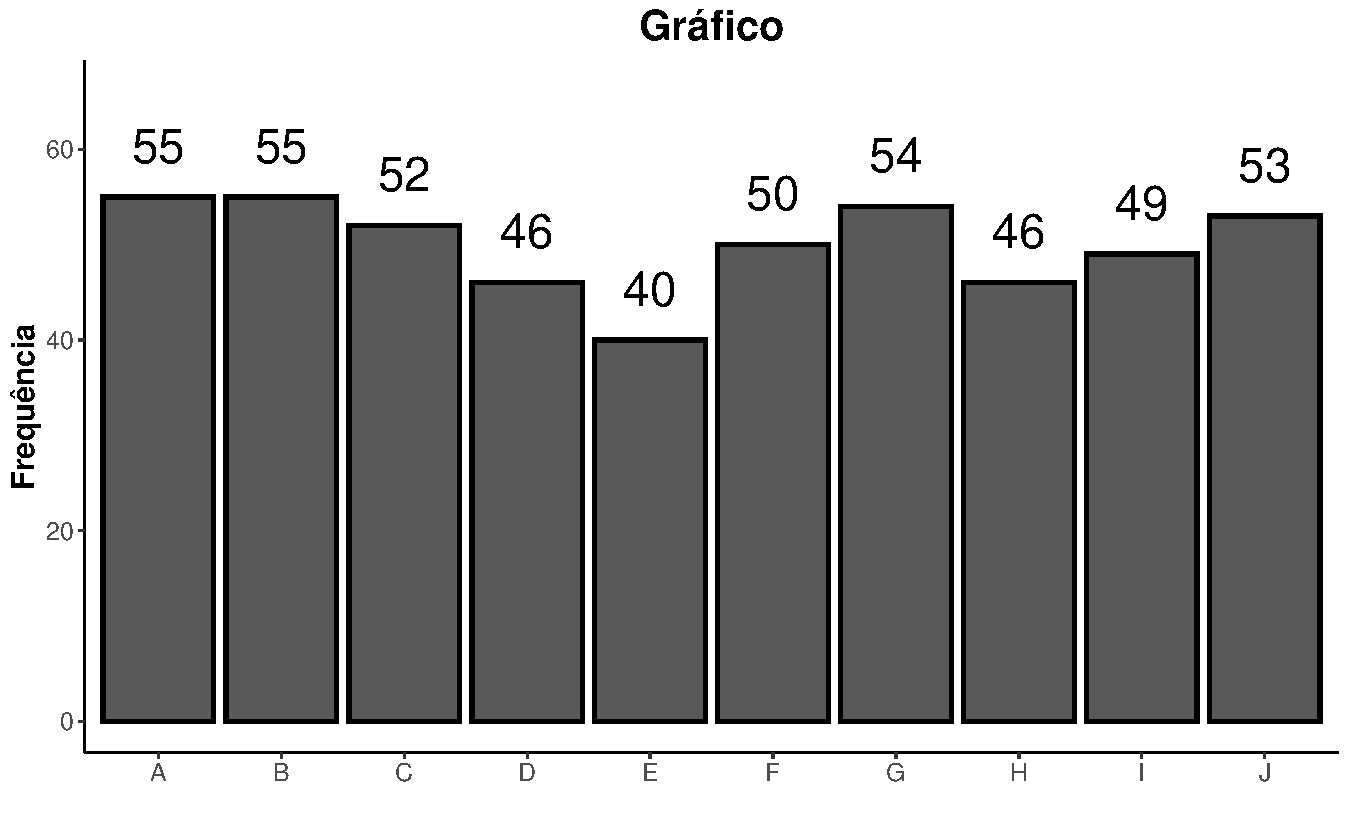
\includegraphics[width=11cm]{200-exploratoria-uni-tabelas-graficos_files/figure-beamer/unnamed-chunk-11-1} 

}

\caption{Gráfico de barras verticais para a variável...}\label{fig:unnamed-chunk-11}
\end{figure}
\end{frame}

\begin{frame}{Gráfico de barras verticais}
\protect\hypertarget{gruxe1fico-de-barras-verticais-1}{}
\begin{figure}

{\centering 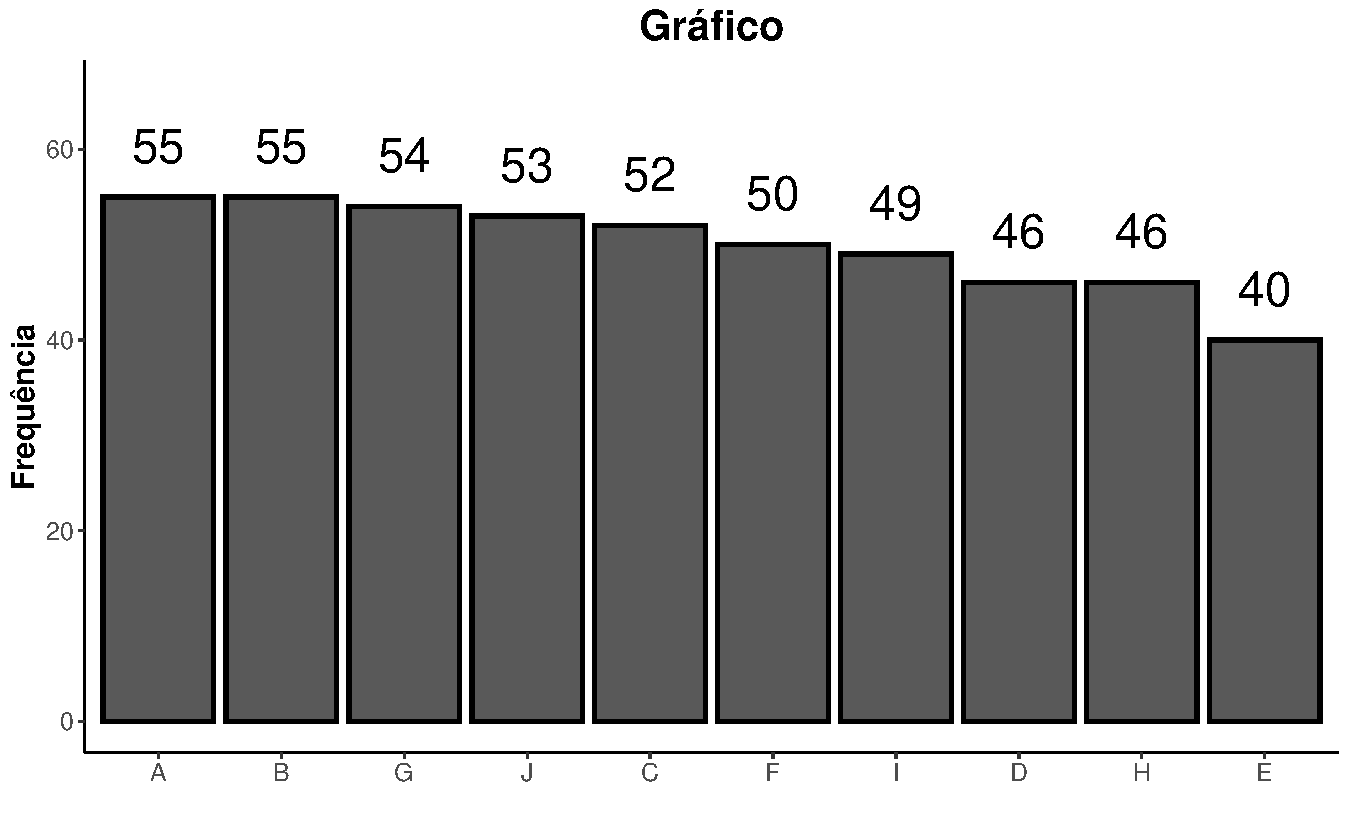
\includegraphics[width=11cm]{200-exploratoria-uni-tabelas-graficos_files/figure-beamer/unnamed-chunk-12-1} 

}

\caption{Gráfico de barras verticais para a variável...}\label{fig:unnamed-chunk-12}
\end{figure}
\end{frame}

\begin{frame}{Gráfico de barras horizontais}
\protect\hypertarget{gruxe1fico-de-barras-horizontais}{}
\begin{figure}

{\centering 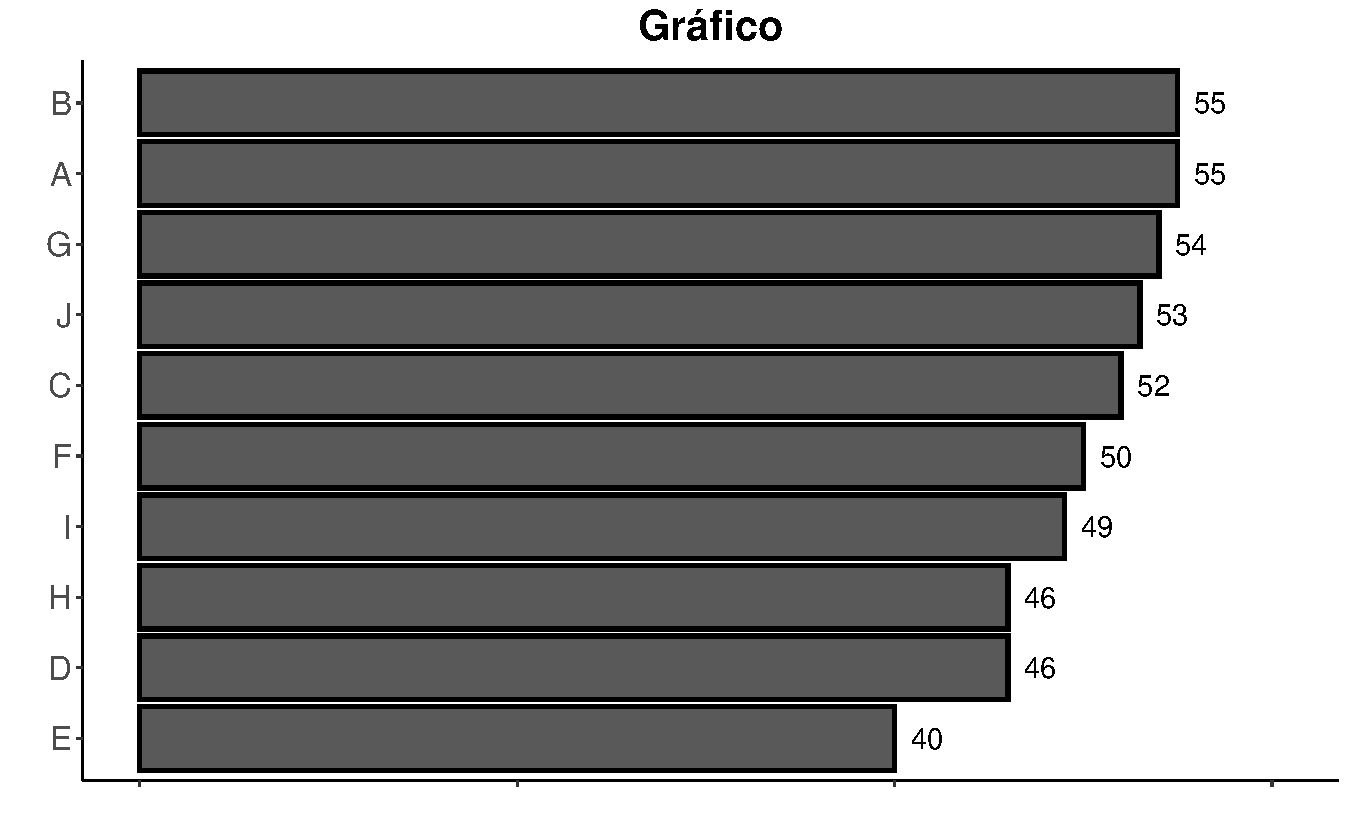
\includegraphics[width=11cm]{200-exploratoria-uni-tabelas-graficos_files/figure-beamer/unnamed-chunk-13-1} 

}

\caption{Gráfico de barras horizontais para a variável...}\label{fig:unnamed-chunk-13}
\end{figure}
\end{frame}

\begin{frame}{Gráfico de barras empilhadas}
\protect\hypertarget{gruxe1fico-de-barras-empilhadas}{}
\begin{figure}

{\centering 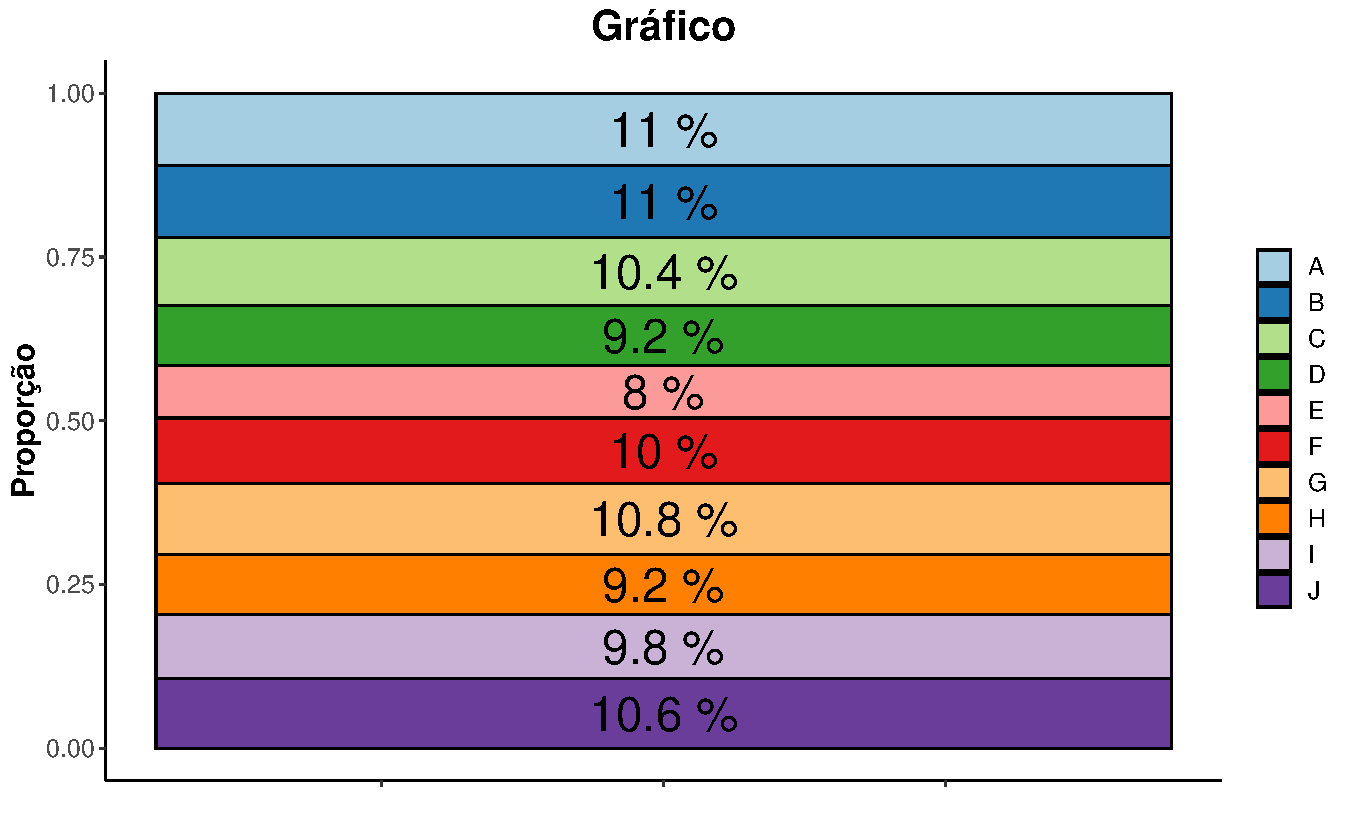
\includegraphics[width=11cm]{200-exploratoria-uni-tabelas-graficos_files/figure-beamer/unnamed-chunk-14-1} 

}

\caption{Gráfico de barras empilhadas para a variável...}\label{fig:unnamed-chunk-14}
\end{figure}
\end{frame}

\begin{frame}{Gráfico de setores}
\protect\hypertarget{gruxe1fico-de-setores}{}
\begin{itemize}
\tightlist
\item
  Consiste em \textbf{repartir um círculo} em setores de tamanhos
  proporcionais às \textbf{frequências relativas} ou às
  \textbf{porcentagens} de cada valor.
\item
  Pode ser usados para representar variáveis com \textbf{poucos níveis}.
\item
  Apesar de muito usado e preferido em diversas áreas, deve ser evitado.
\item
  O cérebro humano tem dificuldade em relacionar frequências com áreas
  relativas.
\item
  Para variáveis com muitos níveis, o gráfico tende a ficar visualmente
  poluído e pouco informativo.
\item
  Outro problema é que níveis com frequências iguais a 0 deixam de
  aparecer no gráfico, diferente de um gráfico de barras.
\end{itemize}
\end{frame}

\begin{frame}{Gráfico de setores}
\protect\hypertarget{gruxe1fico-de-setores-1}{}
\begin{figure}

{\centering 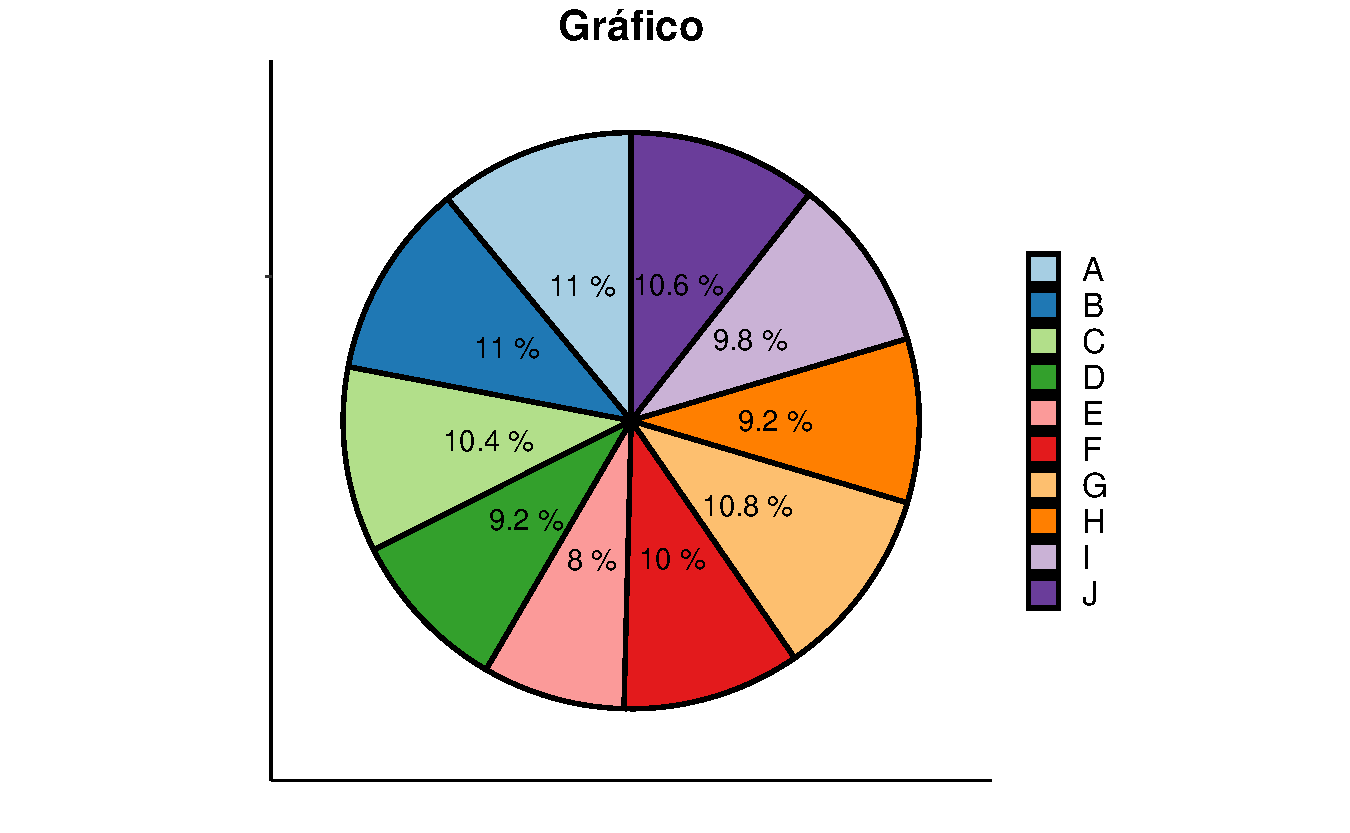
\includegraphics[width=11cm]{200-exploratoria-uni-tabelas-graficos_files/figure-beamer/unnamed-chunk-15-1} 

}

\caption{Gráfico de setores para a variável...}\label{fig:unnamed-chunk-15}
\end{figure}
\end{frame}

\hypertarget{anuxe1lise-descritiva-univariada-para-variuxe1veis-quantitativas}{%
\section{Análise descritiva univariada para variáveis
quantitativas}\label{anuxe1lise-descritiva-univariada-para-variuxe1veis-quantitativas}}

\begin{frame}{Análise descritiva univariada para variáveis
quantitativas}
\protect\hypertarget{anuxe1lise-descritiva-univariada-para-variuxe1veis-quantitativas-1}{}
\begin{itemize}
\item
  Uma variável quantitativa é uma \textbf{característica} que pode ser
  \textbf{representada numericamente}.
\item
  Podem ser classificadas em \textbf{discretas} (finitos valores em um
  dado intervalo) ou \textbf{contínuas} (infinitos valores em um dado
  intervalo).
\item
  Quando estamos lidando com
  \textbf{variáveis quantitativas discretas com poucos possíveis valores},
  as técnicas apresentadas para variáveis qualitativas se aplicam.
\end{itemize}
\end{frame}

\begin{frame}{Tabelas de frequência}
\protect\hypertarget{tabelas-de-frequuxeancia}{}
\begin{longtable}[]{@{}
  >{\centering\arraybackslash}p{(\columnwidth - 8\tabcolsep) * \real{0.1250}}
  >{\centering\arraybackslash}p{(\columnwidth - 8\tabcolsep) * \real{0.1667}}
  >{\centering\arraybackslash}p{(\columnwidth - 8\tabcolsep) * \real{0.1667}}
  >{\centering\arraybackslash}p{(\columnwidth - 8\tabcolsep) * \real{0.2361}}
  >{\centering\arraybackslash}p{(\columnwidth - 8\tabcolsep) * \real{0.3056}}@{}}
\caption{Tabela de frequências para\ldots{}}\tabularnewline
\toprule()
\begin{minipage}[b]{\linewidth}\centering
Valores
\end{minipage} & \begin{minipage}[b]{\linewidth}\centering
Frequência
\end{minipage} & \begin{minipage}[b]{\linewidth}\centering
Percentual
\end{minipage} & \begin{minipage}[b]{\linewidth}\centering
Freq. Acumulada
\end{minipage} & \begin{minipage}[b]{\linewidth}\centering
Percentual Acumulado
\end{minipage} \\
\midrule()
\endfirsthead
\toprule()
\begin{minipage}[b]{\linewidth}\centering
Valores
\end{minipage} & \begin{minipage}[b]{\linewidth}\centering
Frequência
\end{minipage} & \begin{minipage}[b]{\linewidth}\centering
Percentual
\end{minipage} & \begin{minipage}[b]{\linewidth}\centering
Freq. Acumulada
\end{minipage} & \begin{minipage}[b]{\linewidth}\centering
Percentual Acumulado
\end{minipage} \\
\midrule()
\endhead
0 & 47 & 9.4 \% & 47 & 9.4 \% \\
1 & 71 & 14.2 \% & 118 & 23.6 \% \\
2 & 65 & 13 \% & 183 & 36.6 \% \\
3 & 51 & 10.2 \% & 234 & 46.8 \% \\
4 & 54 & 10.8 \% & 288 & 57.6 \% \\
5 & 55 & 11 \% & 343 & 68.6 \% \\
6 & 52 & 10.4 \% & 395 & 79 \% \\
7 & 52 & 10.4 \% & 447 & 89.4 \% \\
8 & 53 & 10.6 \% & 500 & 100 \% \\
Total & 500 & 100 \% & 500 & 100 \% \\
\bottomrule()
\end{longtable}
\end{frame}

\begin{frame}{Gráfico de barras verticais}
\protect\hypertarget{gruxe1fico-de-barras-verticais-2}{}
\begin{figure}

{\centering 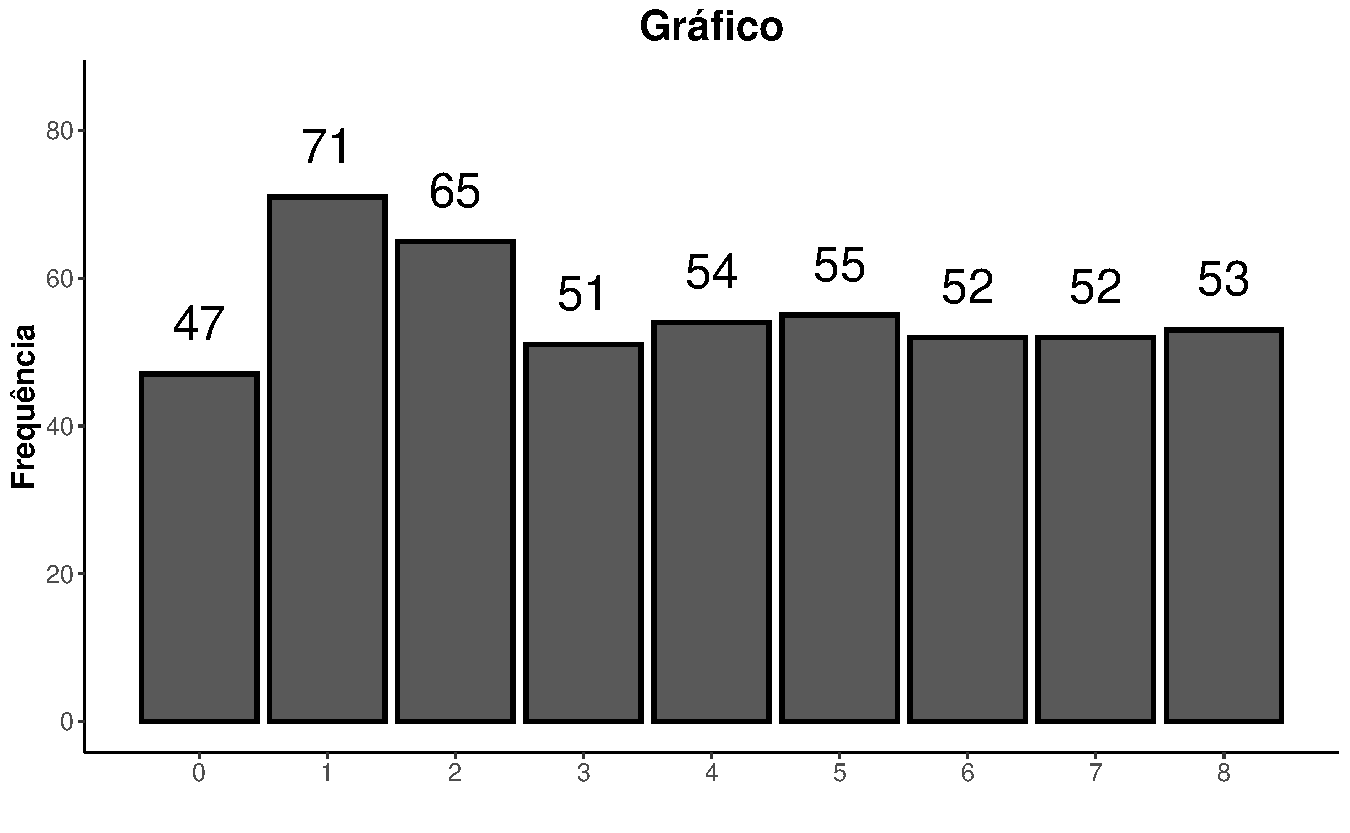
\includegraphics[width=11cm]{200-exploratoria-uni-tabelas-graficos_files/figure-beamer/unnamed-chunk-17-1} 

}

\caption{Gráfico de barras verticais para a variável...}\label{fig:unnamed-chunk-17}
\end{figure}
\end{frame}

\begin{frame}{Análise descritiva univariada para variáveis
quantitativas}
\protect\hypertarget{anuxe1lise-descritiva-univariada-para-variuxe1veis-quantitativas-2}{}
\begin{itemize}
\item
  Para variáveis quantitativas contínuas ou discretas com muitos
  possíveis valores, precisamos de técnicas específicas.
\item
  Uma estratégia comum é o \textbf{agrupamento em faixas de valores}, e
  avaliação das frequências nestas faixas.
\item
  Podem ser usadas tabelas de frequências absolutas, relativas e
  acumuladas para as faixas de valores.
\item
  Utilizando a
  \textbf{razão entre frequência relativa e a amplitude das faixas} de
  valores, geramos a \textbf{densidade}.
\end{itemize}
\end{frame}

\begin{frame}{Análise descritiva univariada para variáveis
quantitativas}
\protect\hypertarget{anuxe1lise-descritiva-univariada-para-variuxe1veis-quantitativas-3}{}
\textbf{Faixas de valores}

\beginAHalfColumn

\begin{itemize}
\item
  Cuidados devem ser tomados quanto às notações e tipos de faixas
  (aberto e fechado à esquerda ou direita).
\item
  Em geral definimos intervalos \textbf{abertos à esquerda} e
  \textbf{fechados à direita}.
\item
  Considerando dois valores \(a\) e \(b\), em que \(a < b\), os
  intervalos consideram que \(a\) \textbf{não} está incluído na faixa,
  \(b\) está.
\end{itemize}

\endColumns
\beginAHalfColumn

\begin{itemize}
\tightlist
\item
  Notações usuais:

  \begin{itemize}
  \tightlist
  \item
    \(a < y \leq b\)
  \item
    \(a \vdash b\)
  \item
    \((a,b]\)
  \end{itemize}
\item
  \(5 < y \leq 10\) ou \(5 \vdash 10\) ou \([5,10)\)

  \begin{itemize}
  \tightlist
  \item
    Valores maiores que 5 até valores menores ou iguais a 10. 5 não está
    no intervalo.
  \end{itemize}
\end{itemize}

\endColumns
\end{frame}

\begin{frame}{Análise descritiva univariada para variáveis
quantitativas}
\protect\hypertarget{anuxe1lise-descritiva-univariada-para-variuxe1veis-quantitativas-4}{}
\begin{itemize}
\item
  Como agrupar em classes?
\item
  Qual o tamanho ideal das faixas de valores?
\item
  Classes definidas com a mesma amplitude é o procedimento mais usual.
\item
  Existem procedimentos que podem ser usados para obter a amplitude,
  como \textbf{Sturges}.
\item
  Em geral, 5 a 15 faixas são suficientes.
\end{itemize}
\end{frame}

\begin{frame}{Tabelas de frequência para uma variável quantitativa}
\protect\hypertarget{tabelas-de-frequuxeancia-para-uma-variuxe1vel-quantitativa}{}
\begin{longtable}[]{@{}
  >{\centering\arraybackslash}p{(\columnwidth - 8\tabcolsep) * \real{0.1184}}
  >{\centering\arraybackslash}p{(\columnwidth - 8\tabcolsep) * \real{0.1579}}
  >{\centering\arraybackslash}p{(\columnwidth - 8\tabcolsep) * \real{0.2105}}
  >{\centering\arraybackslash}p{(\columnwidth - 8\tabcolsep) * \real{0.2237}}
  >{\centering\arraybackslash}p{(\columnwidth - 8\tabcolsep) * \real{0.2895}}@{}}
\caption{Tabela de frequências para\ldots{}}\tabularnewline
\toprule()
\begin{minipage}[b]{\linewidth}\centering
Faixas
\end{minipage} & \begin{minipage}[b]{\linewidth}\centering
Frequência
\end{minipage} & \begin{minipage}[b]{\linewidth}\centering
Freq. Relativa
\end{minipage} & \begin{minipage}[b]{\linewidth}\centering
Freq. Acumulada
\end{minipage} & \begin{minipage}[b]{\linewidth}\centering
Freq. Rel. Acumulada
\end{minipage} \\
\midrule()
\endfirsthead
\toprule()
\begin{minipage}[b]{\linewidth}\centering
Faixas
\end{minipage} & \begin{minipage}[b]{\linewidth}\centering
Frequência
\end{minipage} & \begin{minipage}[b]{\linewidth}\centering
Freq. Relativa
\end{minipage} & \begin{minipage}[b]{\linewidth}\centering
Freq. Acumulada
\end{minipage} & \begin{minipage}[b]{\linewidth}\centering
Freq. Rel. Acumulada
\end{minipage} \\
\midrule()
\endhead
{[}2,4{]} & 1 & 0.002 & 1 & 0.002 \\
(4,6{]} & 46 & 0.092 & 47 & 0.094 \\
(6,8{]} & 102 & 0.204 & 149 & 0.298 \\
(8,10{]} & 111 & 0.222 & 260 & 0.520 \\
(10,12{]} & 111 & 0.222 & 371 & 0.742 \\
(12,14{]} & 82 & 0.164 & 453 & 0.906 \\
(14,16{]} & 27 & 0.054 & 480 & 0.960 \\
(16,18{]} & 15 & 0.030 & 495 & 0.990 \\
(18,20{]} & 3 & 0.006 & 498 & 0.996 \\
(20,22{]} & 2 & 0.004 & 500 & 1.000 \\
\bottomrule()
\end{longtable}
\end{frame}

\begin{frame}{Tabelas de frequência para uma variável quantitativa}
\protect\hypertarget{tabelas-de-frequuxeancia-para-uma-variuxe1vel-quantitativa-1}{}
\begin{longtable}[]{@{}
  >{\centering\arraybackslash}p{(\columnwidth - 8\tabcolsep) * \real{0.1250}}
  >{\centering\arraybackslash}p{(\columnwidth - 8\tabcolsep) * \real{0.1667}}
  >{\centering\arraybackslash}p{(\columnwidth - 8\tabcolsep) * \real{0.1667}}
  >{\centering\arraybackslash}p{(\columnwidth - 8\tabcolsep) * \real{0.2361}}
  >{\centering\arraybackslash}p{(\columnwidth - 8\tabcolsep) * \real{0.3056}}@{}}
\caption{Tabela de frequências para\ldots{}}\tabularnewline
\toprule()
\begin{minipage}[b]{\linewidth}\centering
Faixas
\end{minipage} & \begin{minipage}[b]{\linewidth}\centering
Frequência
\end{minipage} & \begin{minipage}[b]{\linewidth}\centering
Percentual
\end{minipage} & \begin{minipage}[b]{\linewidth}\centering
Freq. Acumulada
\end{minipage} & \begin{minipage}[b]{\linewidth}\centering
Percentual Acumulado
\end{minipage} \\
\midrule()
\endfirsthead
\toprule()
\begin{minipage}[b]{\linewidth}\centering
Faixas
\end{minipage} & \begin{minipage}[b]{\linewidth}\centering
Frequência
\end{minipage} & \begin{minipage}[b]{\linewidth}\centering
Percentual
\end{minipage} & \begin{minipage}[b]{\linewidth}\centering
Freq. Acumulada
\end{minipage} & \begin{minipage}[b]{\linewidth}\centering
Percentual Acumulado
\end{minipage} \\
\midrule()
\endhead
{[}2,4{]} & 1 & 0.2 \% & 1 & 0.2 \% \\
(4,6{]} & 46 & 9.2 \% & 47 & 9.4 \% \\
(6,8{]} & 102 & 20.4 \% & 149 & 29.8 \% \\
(8,10{]} & 111 & 22.2 \% & 260 & 52 \% \\
(10,12{]} & 111 & 22.2 \% & 371 & 74.2 \% \\
(12,14{]} & 82 & 16.4 \% & 453 & 90.6 \% \\
(14,16{]} & 27 & 5.4 \% & 480 & 96 \% \\
(16,18{]} & 15 & 3 \% & 495 & 99 \% \\
(18,20{]} & 3 & 0.6 \% & 498 & 99.6 \% \\
(20,22{]} & 2 & 0.4 \% & 500 & 100 \% \\
\bottomrule()
\end{longtable}
\end{frame}

\begin{frame}{Tabelas de frequência para uma variável quantitativa}
\protect\hypertarget{tabelas-de-frequuxeancia-para-uma-variuxe1vel-quantitativa-2}{}
\begin{longtable}[]{@{}
  >{\centering\arraybackslash}p{(\columnwidth - 12\tabcolsep) * \real{0.1111}}
  >{\centering\arraybackslash}p{(\columnwidth - 12\tabcolsep) * \real{0.1481}}
  >{\centering\arraybackslash}p{(\columnwidth - 12\tabcolsep) * \real{0.1481}}
  >{\centering\arraybackslash}p{(\columnwidth - 12\tabcolsep) * \real{0.1605}}
  >{\centering\arraybackslash}p{(\columnwidth - 12\tabcolsep) * \real{0.1605}}
  >{\centering\arraybackslash}p{(\columnwidth - 12\tabcolsep) * \real{0.1358}}
  >{\centering\arraybackslash}p{(\columnwidth - 12\tabcolsep) * \real{0.1358}}@{}}
\caption{Tabela de frequências para\ldots{}}\tabularnewline
\toprule()
\begin{minipage}[b]{\linewidth}\centering
Faixas
\end{minipage} & \begin{minipage}[b]{\linewidth}\centering
Frequência
\end{minipage} & \begin{minipage}[b]{\linewidth}\centering
Percentual
\end{minipage} & \begin{minipage}[b]{\linewidth}\centering
Freq. Acum.
\end{minipage} & \begin{minipage}[b]{\linewidth}\centering
Perc. Acum.
\end{minipage} & \begin{minipage}[b]{\linewidth}\centering
Amplitude
\end{minipage} & \begin{minipage}[b]{\linewidth}\centering
Densidade
\end{minipage} \\
\midrule()
\endfirsthead
\toprule()
\begin{minipage}[b]{\linewidth}\centering
Faixas
\end{minipage} & \begin{minipage}[b]{\linewidth}\centering
Frequência
\end{minipage} & \begin{minipage}[b]{\linewidth}\centering
Percentual
\end{minipage} & \begin{minipage}[b]{\linewidth}\centering
Freq. Acum.
\end{minipage} & \begin{minipage}[b]{\linewidth}\centering
Perc. Acum.
\end{minipage} & \begin{minipage}[b]{\linewidth}\centering
Amplitude
\end{minipage} & \begin{minipage}[b]{\linewidth}\centering
Densidade
\end{minipage} \\
\midrule()
\endhead
{[}2,4{]} & 1 & 0.2 \% & 1 & 0.2 \% & 2 & 0.001 \\
(4,6{]} & 46 & 9.2 \% & 47 & 9.4 \% & 2 & 0.046 \\
(6,8{]} & 102 & 20.4 \% & 149 & 29.8 \% & 2 & 0.102 \\
(8,10{]} & 111 & 22.2 \% & 260 & 52 \% & 2 & 0.111 \\
(10,12{]} & 111 & 22.2 \% & 371 & 74.2 \% & 2 & 0.111 \\
(12,14{]} & 82 & 16.4 \% & 453 & 90.6 \% & 2 & 0.082 \\
(14,16{]} & 27 & 5.4 \% & 480 & 96 \% & 2 & 0.027 \\
(16,18{]} & 15 & 3 \% & 495 & 99 \% & 2 & 0.015 \\
(18,20{]} & 3 & 0.6 \% & 498 & 99.6 \% & 2 & 0.003 \\
(20,22{]} & 2 & 0.4 \% & 500 & 100 \% & 2 & 0.002 \\
\bottomrule()
\end{longtable}
\end{frame}

\begin{frame}{Gráficos para representação de frequências de uma variável
quantitativa}
\protect\hypertarget{gruxe1ficos-para-representauxe7uxe3o-de-frequuxeancias-de-uma-variuxe1vel-quantitativa}{}
\beginAHalfColumn

\begin{itemize}
\tightlist
\item
  Assim como no caso de variáveis qualitativas ou quantitativas
  discretas com poucos possíveis valores, a representação por meio de
  gráficos pode ser bastante benéfica para análise de variáveis
  quantitativas.
\end{itemize}

\endColumns
\beginAHalfColumn

Algumas possibilidades são

\begin{itemize}
\tightlist
\item
  Histograma.
\item
  Gráfico de densidade empírica.
\item
  Box-plot
\end{itemize}

\endColumns
\end{frame}

\begin{frame}{Histograma}
\protect\hypertarget{histograma}{}
\begin{itemize}
\item
  Consiste em \textbf{retângulos contíguos} de base dada pelas faixas de
  valores definindas para uma variável.
\item
  Algumas possibilidades são:

  \begin{itemize}
  \tightlist
  \item
    A área representar a frequência da rescpectiva faixa.
  \item
    A altura representar a frequência absoluta na faixa.
  \item
    A altura representar o quociente da área pela amplitude da faixa: a
    densidade.
  \end{itemize}
\end{itemize}
\end{frame}

\begin{frame}{Histograma}
\protect\hypertarget{histograma-1}{}
\begin{figure}

{\centering 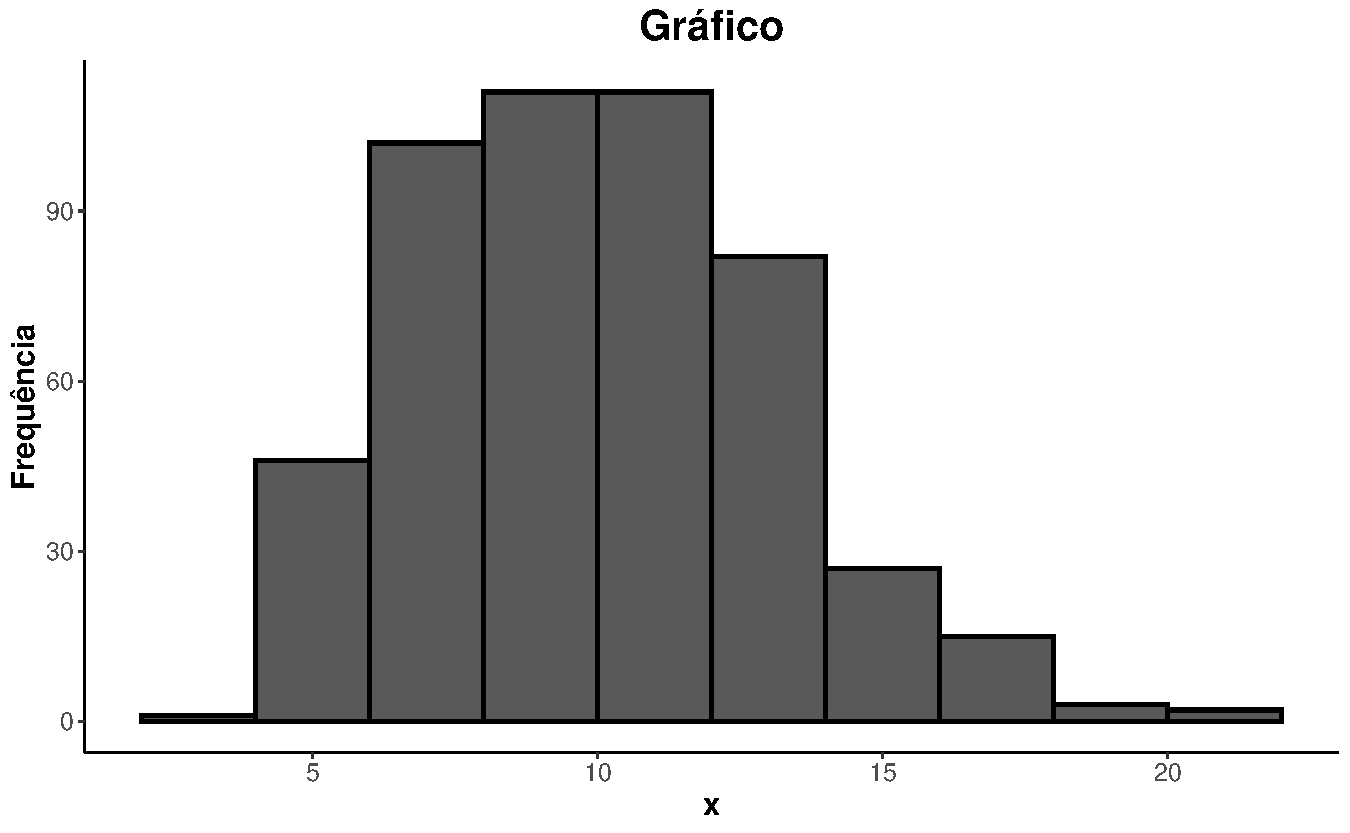
\includegraphics[width=11cm]{200-exploratoria-uni-tabelas-graficos_files/figure-beamer/unnamed-chunk-21-1} 

}

\caption{Gráfico de setores para a variável...}\label{fig:unnamed-chunk-21}
\end{figure}
\end{frame}

\begin{frame}{Efeito do número de classes}
\protect\hypertarget{efeito-do-nuxfamero-de-classes}{}
\begin{itemize}
\item
  O número de classes pode afetar diretamente as tabelas e gráficos.
\item
  Com poucas classes, os dados ficam excessivamente resumidos e as
  classes ficam muito heterogêneas.
\item
  Com muitas classes, os dados ficam segmentados em excesso e as
  representações são comprometidas.
\end{itemize}
\end{frame}

\begin{frame}{Efeito do número de classes}
\protect\hypertarget{efeito-do-nuxfamero-de-classes-1}{}
\begin{figure}

{\centering 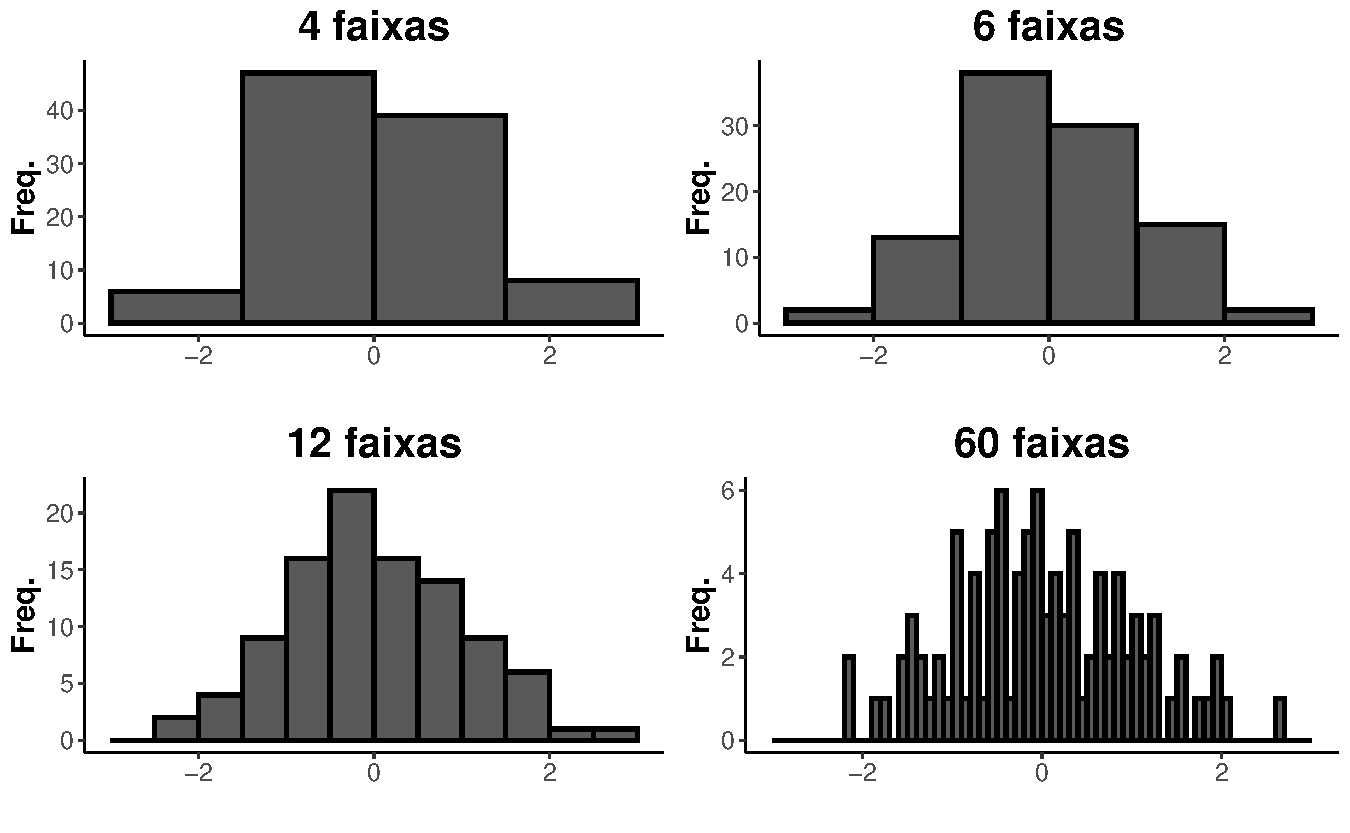
\includegraphics[width=11cm]{200-exploratoria-uni-tabelas-graficos_files/figure-beamer/unnamed-chunk-22-1} 

}

\caption{Gráfico de setores para a variável...}\label{fig:unnamed-chunk-22}
\end{figure}
\end{frame}

\begin{frame}{Gráfico de densidade empírica}
\protect\hypertarget{gruxe1fico-de-densidade-empuxedrica}{}
\beginAHalfColumn

\textbf{Intuição}

\begin{itemize}
\item
  Imagine uma sequência de histogramas de densidade em que o número de
  observações aumenta, juntamente com o número de faixas.
\item
  No limite, teremos uma curva.
\item
  Esta curva é chamada de gráfico de densidade empírica.
\item
  É um gráfico ``computacionalmente intensivo'', depende da definição de
  uma função kernel e do tamanho da banda.
\item
  A área sob a curva é igual a 1.
\end{itemize}

\endColumns
\beginAHalfColumn

\begin{figure}

{\centering 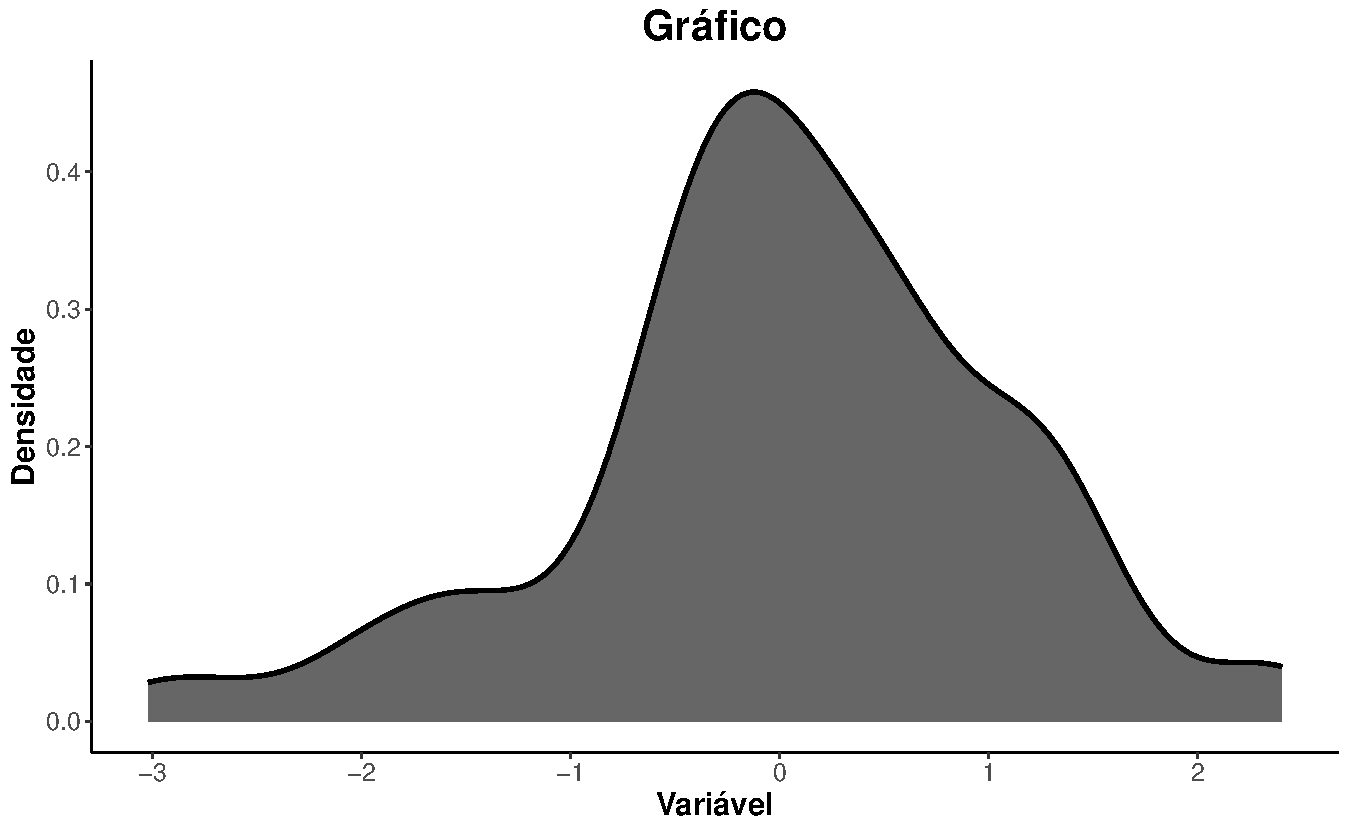
\includegraphics[width=1\linewidth]{200-exploratoria-uni-tabelas-graficos_files/figure-beamer/unnamed-chunk-23-1} 

}

\caption{Gráfico de setores para a variável...}\label{fig:unnamed-chunk-23}
\end{figure}

\endColumns
\end{frame}

\begin{frame}{Box-plot}
\protect\hypertarget{box-plot}{}
\begin{itemize}
\item
  Outra importante visualização é o box-plot.
\item
  É possível analisar a distribuição dos dados, aspectos quanto a
  posição, variabilidade, assimetria e também a presença de valores
  atípicos.
\item
  Retomaremos o box-plot após estudar quartis, em medidas descritivas.
\end{itemize}

\begin{figure}

{\centering 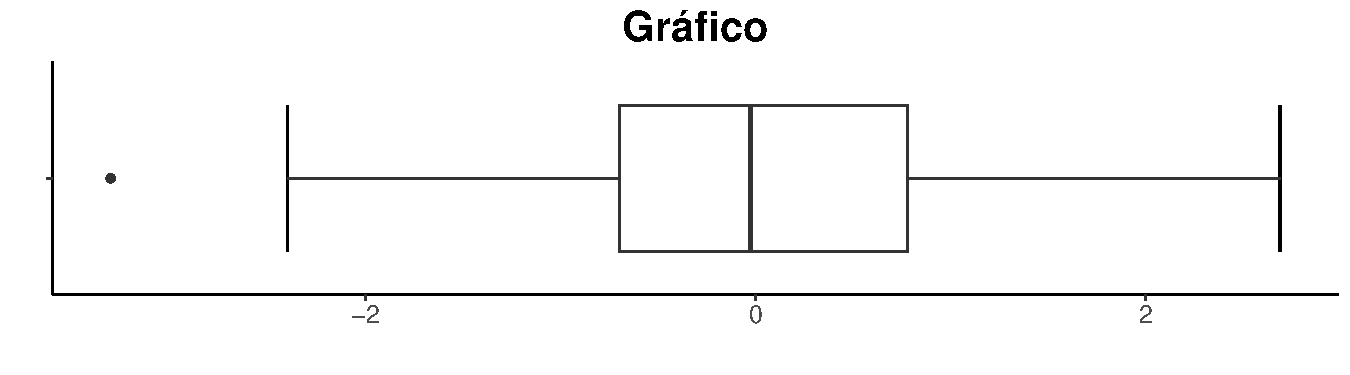
\includegraphics[width=11cm]{200-exploratoria-uni-tabelas-graficos_files/figure-beamer/unnamed-chunk-24-1} 

}

\caption{Gráfico de setores para a variável...}\label{fig:unnamed-chunk-24}
\end{figure}
\end{frame}

\begin{frame}{Histograma, densidade e box-plot}
\protect\hypertarget{histograma-densidade-e-box-plot}{}
\begin{figure}

{\centering 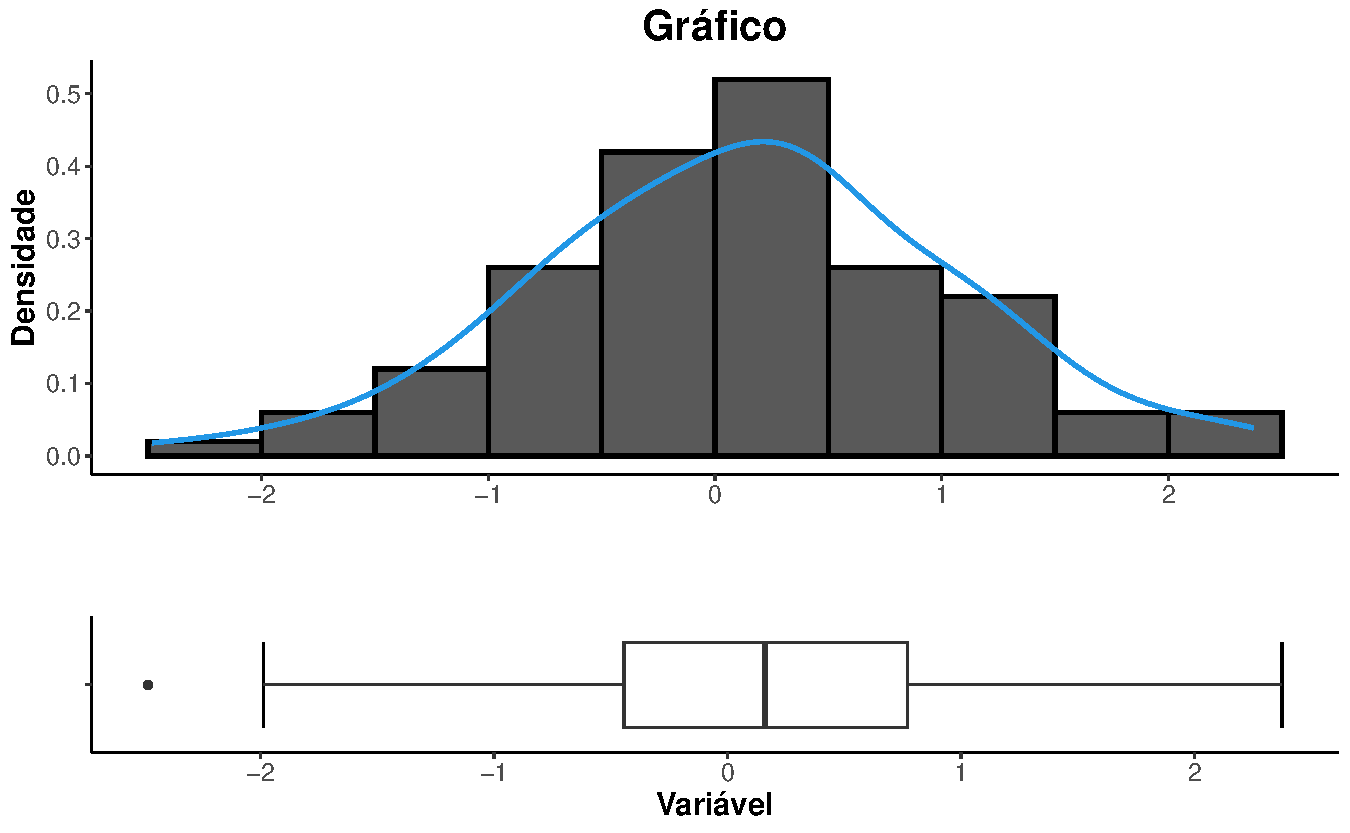
\includegraphics[width=11cm]{200-exploratoria-uni-tabelas-graficos_files/figure-beamer/unnamed-chunk-25-1} 

}

\caption{Gráfico de setores para a variável...}\label{fig:unnamed-chunk-25}
\end{figure}
\end{frame}

\begin{frame}{Assimetria}
\protect\hypertarget{assimetria}{}
\begin{itemize}
\item
  Um conjunto pode ser aproximadamente \textbf{simétrico},
  \textbf{assimétrico} à esquerda ou à direita.
\item
  Tais características são facilmente diagnosticadas por meio de análise
  gráfica usando um histograma, gráfico de densidade ou box-plot.
\item
  Futuramente veremos como diagnosticar assimetria por meio de medidas
  descritivas.
\end{itemize}

\begin{figure}

{\centering 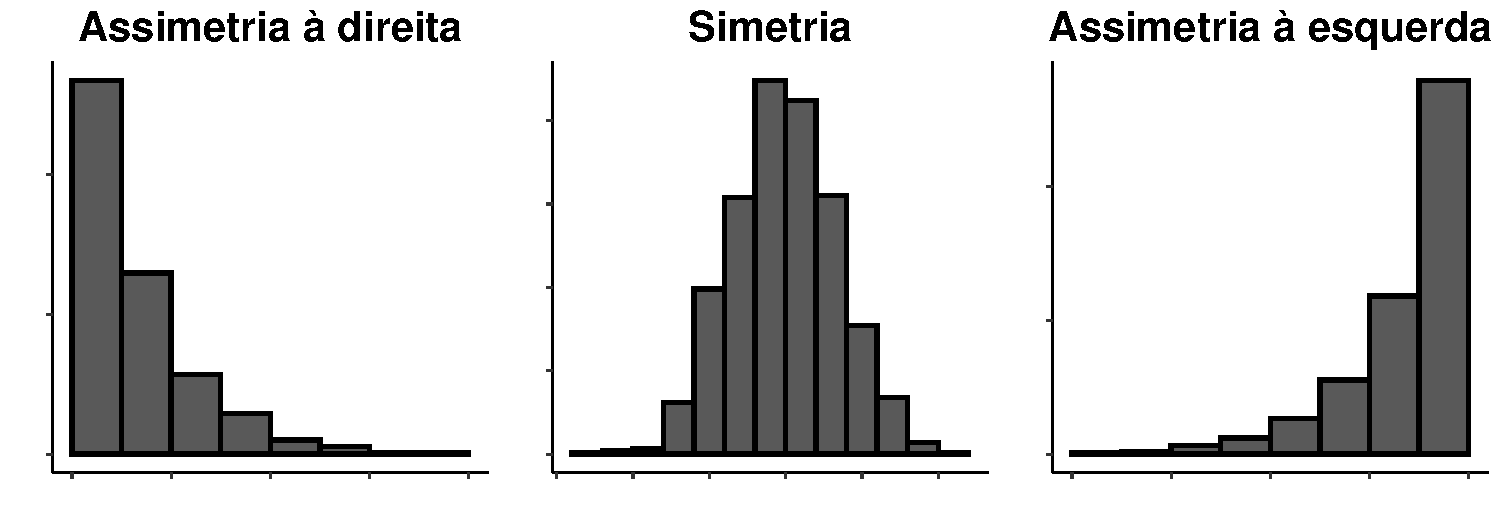
\includegraphics[width=11cm]{200-exploratoria-uni-tabelas-graficos_files/figure-beamer/unnamed-chunk-26-1} 

}

\caption{Gráfico de setores para a variável...}\label{fig:unnamed-chunk-26}
\end{figure}
\end{frame}

\begin{frame}{}
\protect\hypertarget{section}{}
\beginAHalfColumn

\textbf{O que foi visto:}

\begin{itemize}
\tightlist
\item
  Introdução à análise exploratória.
\item
  Análise exploratória univariada para variáveis qualitativas.
\item
  Análise exploratória univariada para variáveis quantitativas.
\end{itemize}

\endColumns
\beginAHalfColumn

\textbf{Próximos assuntos:}

\begin{itemize}
\tightlist
\item
  Resumos numéricos.
\item
  Medidas de posição central.
\item
  Medidas de posição relativa.
\item
  Medidas de dispersão.
\end{itemize}

\endColumns
\end{frame}

\end{document}
